\documentclass[journal]{IEEEtran}
\usepackage{ragged2e}
\usepackage{subcaption}
\usepackage{amsmath,amsthm,amssymb,mathtools}
\usepackage{amsmath}
\usepackage{amsthm}
\newtheorem{theorem}{Theorem}[section]
\newtheorem{lemma}[theorem]{Lemma}
\usepackage{amssymb}
\usepackage{todonotes}
\usepackage[author={Amirhossein Tamjidi}]{pdfcomment}
\usepackage{balance}

\DeclareFontFamily{OT1}{pzc}{}
\DeclareFontShape{OT1}{pzc}{m}{it}{<-> s * [1.10] pzcmi7t}{}
\DeclareMathAlphabet{\mathpzc}{OT1}{pzc}{m}{it}
\DeclareMathOperator*{\argmin}{argmin}  
\usepackage{xifthen}
\usepackage{hyperref}
\usepackage[normalem]{ulem}
\usepackage{xcolor}
\hypersetup{
colorlinks,
linkcolor={red!50!black},
citecolor={blue!50!black},
urlcolor={blue!80!black}
}
\usepackage{xparse}
%\newcommand{\vect}{\bf}
\newcommand{\vect}[1]{{\mathbf{#1}}}
\newcommand{\matr}{\bf}
\newcommand{\net}{\ensuremath{\textsc{net}}}

\newtheorem{prop}{Proposition}
\theoremstyle{remark}
\newtheorem{remark}{Remark}
\usepackage{pgfplots} 
\newlength\figureheight 
\newlength\figurewidth
\pgfplotsset{compat=newest} 
\pgfplotsset{plot coordinates/math parser=false} 
%\renewcommand{\footnotesize}{\footnotesize}
\renewcommand{\footnotesize}{\fontsize{7.5pt}{9pt}\selectfont}
%\usepackage{enumitem}

\newcommand{\TODO}[1]{{\color{orange}{#1}}}  % Typo or 
\newcommand{\DONE}[1]{{\color{blue}{#1}}}  % Typo or 
\newcommand{\AMIR}[1]{{\color{green}{#1}}}  % Typo or 
%\newcommand{\bIn}{\boldsymbol{I}_{\boldsymbol{n}}}
%\newcommand{\bIa}{\boldsymbol{I}_{\boldsymbol{a}}}
%\newcommand{\bIk}{\boldsymbol{I}_{\boldsymbol{k}}}
%\newcommand{\bIkk}{\boldsymbol{I}_{\boldsymbol{k-1}}}

\newcommand{\pr}{\textrm{p}}
\newcommand{\XX}[3][2]{\mathbf{X}_{  #2}^{ #3}}

\newcommand{\bIn}{\boldsymbol{I}_{{n}}}
\newcommand{\bIa}{\boldsymbol{I}_{{a}}}
\newcommand{\bIk}{\boldsymbol{I}_{{k}}}
\newcommand{\bIkk}{\boldsymbol{I}_{{k-1}}}
\newcommand{\bIs}[1]{\boldsymbol{I}_{#1}}  % Suman's comments
\newcommand{\xx}[3][2]{\mathbf{x}_{ #2}^{ #3}}
\newcommand{\zz}[3][2]{\mathbf{z}_{ #2}^{ #3}}
\newcommand{\ZZ}[3][2]{\mathbf{Z}_{ #2}^{ #3}}
\newcommand{\ZZh}[3][2]{\mathbf{\hat{z}}_{ #2}^{ #3}}
%\newcommand{\yy}[3][2]{\mathpzc{y}_{\tiny #2}^{\tiny #3}}
%\newcommand{\YY}[3][2]{\mathpzc{Y}_{\tiny #2}^{\tiny #3}}

\newcommand{\yy}[3][2]{\psi^{  #3}({  #2})}
\newcommand{\YY}[3][2]{\phi^{  #3}({  #2})}
\newcommand{\suf}[1]{\textsc{\tiny #1}}  % Suman's comments

\newcommand{\ii}[3][2]{\overline{\delta \mathpzc{i}}_{\tiny {#2}}^{\tiny {#3}}}
\newcommand{\II}[3][2]{\overline{\delta \mathpzc{I}}_{\tiny {#2}}^{\tiny {#3}}}
\newcommand{\psx}{p_*(\vect{x})}
\newcommand{\pcfx}{p_{\textsc{\tiny CF}}(\vect{x})}
\newcommand{\phybx}{p_{\textsc{\tiny HYB}}(\vect{x})}
\newcommand{\pixz}{\tilde{p}^i(\xx[]{k}{}\vert \vect{Z}_{k})}
\newcommand{\pixzm}{\tilde{p}^i(\xx[]{k}{}\vert \vect{Z}_{k-1})}
\newcommand{\pzix}{\tilde{p}^i( \vect{z}_{k} \vert \xx[]{k}{})}
\newcommand{ \pcf}{\frac{1}{\eta_{\textsuperscript{ICF}}}\prod_{i=1}^{N} \pr(\vect{z}_{k}^i | \xx[]{k}{})^{\omega_i} \prod_{i=1}^{N} \tilde{p}^i(\vect{x}_{k} | \vect{Z}_{k-1})^{\omega_i}}
\newcommand{ \phyb}{\frac{1}{\eta_{\textsc{\tiny HYB}}}\prod_{i=1}^{N} \pr(\vect{z}_{k}^i | \xx[]{k}{}) \prod_{i=1}^{N} \tilde{p}^i(\vect{x}_{k} | \vect{Z}_{k-1})^{\bar{\omega}_i} }
\newcommand{ \pstar}{\frac{1}{\eta_*} \{ \prod_{i=1}^{N} \pr(\vect{z}_{k}^i | \xx[]{k}{}) \} \pr(\xx[]{k}{}|\vect{Z}_{k-1})}

\newcommand{ \npcf}{\prod_{i=1}^{N} \pr(\vect{z}_{k}^i | \xx[]{k}{})^{\omega_i} \prod_{i=1}^{N} \tilde{p}^i(\vect{x}_{k} | \vect{Z}_{k-1})^{\omega_i}}
\newcommand{ \nphyb}{\prod_{i=1}^{N} \pr(\vect{z}_{k}^i | \xx[]{k}{}) \prod_{i=1}^{N} \tilde{p}^i(\vect{x}_{k} | \vect{Z}_{k-1})^{\bar{\omega}_i} }
\newcommand{ \npstar}{ \{ \prod_{i=1}^{N} \pr(\vect{z}_{k}^i | \xx[]{k}{}) \} \pr(\xx[]{k}{}|\vect{Z}_{k-1})}

\DeclareDocumentCommand{\ais}{m m m  }{{#1}_{#2}^{#3}}
\DeclareDocumentCommand{\bis}{m m m  }{{#1}_{{\tiny #2}}^{{\tiny #3}}}
\DeclareDocumentCommand{\cis}{m m m  }{{#1}_{{\tiny #2}}^{{\tiny {#3}}}}
\newcommand{\ti}[1]{\textsc{\tiny #1}}
\newcommand{\lrp}[1]{\left( #1 \right) }

\allowdisplaybreaks[1]

\usepackage[linesnumbered]{algorithm2e}
\usepackage{algpseudocode}
\usepackage{microtype}
\usepackage{lipsum}
\usepackage[utf8]{inputenc}

\theoremstyle{definition}
\newtheorem{definition}{Definition}[section]


\title{\LARGE \bf Efficient Recursive Distributed State Estimation of\\ Hidden Markov Models over Unreliable
Networks}
\author {Amirhossein Tamjidi$^{1}$, Reza Oftadeh$^{2}$, Suman Chakravorty$^{1}$, and Dylan Shell$^{2}$
\thanks{$^{1}$Department of Aerospace Engineering, Texas A\&M University}
\thanks{$^{2}$Department of Computer Science \& Engineering, Texas A\&M University}
\thanks{Corresponding author email: ahtamjidi@tamu.edu}}

\begin{document}

\maketitle

\begin{abstract}
A new recursive consensus filter for distributed state estimation on Hidden
Markov Models (HMMs) is presented and shown to be well-suited to multi-robot
settings and associated applications.  The algorithm is scalable, robust to
network failure, capable of handling non-Gaussian transition and observation
models, and is, therefore, quite general.  Crucially, no global knowledge of
the communication network is assumed.  The algorithm is a Hybrid method:
Iterative Conservative Fusion (ICF) is used to reach consensus over potentially
correlated priors, while consensus over likelihoods is handled using weights
based on a Metropolis Hastings Markov Chain (MHMC).  To attain a detailed
understanding of the theoretical upper limit for estimator performance modulo
imperfect communication, we introduce an idealized distributed estimator.  It
is shown that under certain general conditions, the Hybrid method converges
exponentially to the ideal distributed estimator, despite the latter being
conceptual and utterly unworkable in practice.  The method is extensively
evaluated in a series of simulated experiments and its performance surpasses
competing algorithms.
\end{abstract}

\section{Introduction}
Mobile and robotic-sensor networks have many applications and the problem of
estimation within such networks has, thus, been a topic of extensive study in
recent
years~\cite{durrant2001data,campbell2016distributed,boem2015decentralized}.  In
a robotic-sensor network, robots carry sensors that make noisy observations of
the state of an underlying system of interest. Their estimation process is
considered centralized if all the nodes send their raw observations to a
central node that is responsible for calculating an estimate based on the
collective information~\cite{ahmed201522}. This is not always possible owing to
link failures as well as bandwidth and energy
constraints~\cite{Zhang_ttradeof1}. 

One alternative\,---which we term distributed state estimation (DSE)---\,is to
adopt a message passing protocol between agents and strive to achieve the same
result as the centralized estimation via a distributed process.  In order to be
viable, if messages are to contain raw information, the fundamental challenge
is to identify and account for mutual information before passing a message from
one agent to another. The Channel Filter~\cite{durrant2001data}, a classic
method in this category, presupposes a directed communication network topology
and relies on bookkeeping to make sure no information is double counted during
message passing. The Channel Filter can fully recover the performance of the
centralized estimator so long as the network is fully connected and time
invariant. A similar bookkeeping-based approach, but which  relaxes the
directed communication graph requirement, was proposed by Bahr, Walter and
Leonard~\cite{bahr09consistent}. Their method keeps track of the provenance of
individual measurements to avoid double counting.  The final estimates produced
are conservative and consistent approximations of the centralized approach and
their method outperforms other conservative fusion DSE approaches that do not
perform bookkeeping. However, the basic problem with DSE methods that rely on
bookkeeping is their inability to scale.  The information being maintained is
inherently combinatorial in nature, so they are unsuitable for large-scale
networks and their resource requirements (usually for CPU or memory, but
possibly communication as well) can be prohibitive even in networks of moderate
size.

Most DSE research in recent years has focused on approaches that rely on
consensus methods.  The objective then becomes to design both a protocol for
message passing between nodes and local fusion rules so that the nodes reach a
consensus over their collective information.  Although DSE algorithms are not
guaranteed to match the performance of the centralized estimator all the time,
their scalability, modularity, and robustness to network failure have fueled
interest in the approach. These features are important in the
applications envisioned for robots employing such algorithms, such as
multi-agent localization~\cite{simonetto10distributed}.

Categorizing DSE methods on the basis of the
modeling assumptions they make gives a 
useful miniature taxonomy of algorithms. Any DSE method makes assumptions about one or
more of the following aspects: the state (static~\cite{xiao2005scheme} \emph{vs.}
dynamic~\cite{simonetto10distributed}), state transition model
(linear~\cite{olfati2005distributed} \emph{vs.}
nonlinear~\cite{battistelli2014parallel,rao2003constrained,boem2013distributed,hu2014state}),
type of noise (Gaussian~\cite{xiao2005scheme,olfati2005distributed} \emph{vs.}
non-Gaussian~\cite{hlinka2013distributed}), topology of the network (constant
\emph{vs.} changing~\cite{tamjidi2016unifying,xiao2005scheme}), connectivity of the
network (persistent~\cite{battistelli2014parallel} \emph{vs.}
intermittent~\cite{tamjidi2016unifying,xiao2005scheme}), the agents' knowledge
of the network topology (global \emph{vs.} local
\cite{tamjidi2016unifying,xiao2005scheme,battistelli2014parallel}) and finally
the treatment of mutual information between estimates (exact solution through
bookkeeping \cite{durrant2001data} \emph{vs.} conservative solutions that avoid double
counting \cite{wang_distr_CI,hu2012diffusion}).

The research on DSE for linear systems with Gaussian noise is extensive
(see~\cite{olfati2005distributed} and~\cite{cattivelli2010diffusion} for
reviews).  For nonlinear systems with Gaussian noise, the distributed versions
of Extended Kalman Filters (EKF)~\cite{battistelli2016stability,
 battistelli2014parallel}, Extended Information Filters
(EIF)~\cite{dist_inf_filter_2009} and Unscented Kalman Filter
(UKF)~\cite{niu2017distributed} have been proposed.  For nonlinear systems with
non-Gaussian noise, different variants of Distributed Particle Filter (DPF)
methods have also been proposed~\cite{lin_dist_part_filter_2014}. 

For dynamic state systems within time-varying networks, the connectivity
constraint is a determining factor for choosing the proper DSE method. If the
network remains connected, DSE methods can maintain equality of each node's
priors and then keep the likelihoods identical by performing consensus on the
likelihoods~\cite{hlinka2012likelihood,li2012distributed}.  We refer to this
approach as Consensus on Likelihoods (CL). The advantage of CL is that, given
sufficient time to reach consensus, it can match the centralized estimator's
performance.  However, if the network becomes disconnected, or if the  consensus steps are limited, the priors start to
depart from one another. Once the priors differ across nodes, CL methods will
fail.

In the case of disparities between priors owing to network disconnection, the
prevailing fix is an approach where the agent's perform Iterative Conservative
Fusion (ICF) on node
posteriors~\cite{battistelli2014kullback,wang_distr_CI,hu2012diffusion}. Such
ICF methods have a conservative fusion rule that avoids double counting at the
expense of down weighting the uncorrelated information. As a consequence they
are inherently sub-optimal.
In the case of disparities between prior owing to early termination 
of a consensus process, \cite{battistelli2014parallel} and~\cite{battistelli2016stability} proposed to use a
combination of CL and ICF. To justify their method they refer to the complimentary
features of CL and ICF. They claim that ICF underweights the new information
and showed better performance when very few consensus iterations have been 
executed. On the other hand, CL takes longer to converge but can recover the
centralized estimator's performance. Therefore, when the number of consensus
iterations are limited, the proposed combination can bring about the
complementary benefits of both of them. 

The precedence of \cite{battistelli2014parallel}
and~\cite{battistelli2016stability} in their amalgamation of CL and ICF must be
acknowledged openly: the present authors were working on the method described herein,
albeit with the distinct motive of developing approaches to operate under
conditions of severe network degradation, and encountered their work only after
our first publication on the subject~\cite{tamjidi2016unifying}.  In essence,
our assumptions on the network are different and, consequently, the analysis
and final results are different from~\cite{battistelli2014parallel, battistelli2016stability}. (In detail  Proposition~\ref{prop:netperf} yields the quality of network necessary to
achieve some desired performance---a question that is only meaningful when the
network is not assumed to be fully connected, as was assumed
in~\cite{battistelli2014parallel, battistelli2016stability}.) Our viewpoint is
that network disconnection will inevitably result in unequal priors and using
ICF alone will mean that much of the new information, despite being
uncorrelated, will be diluted in the consensus process.  However, handling
priors with ICF and new information with CL reaps the benefits and, as we will
show, the performance in settings where the communication network is unreliable
is outstanding---so good in fact as to eclipse previously envisioned domains of
applicability.

\TODO{THIS CAN BE PLACED HERE OR PREFERABLY TO DISCUSSION/CONCLUSION SECTION} \AMIR{For application purposes it is worth clarifying what is the difference between the underlying method of this paper and \cite{battistelli2014parallel} and when one should opt for either of them. In terms of underlying approach, both methods follow the same fusion rules for independent and correlation sources of information. This paper fleshes out the realization of fusion rules for discrete case while \cite{battistelli2014parallel} details the implementation for continuous linear and non-linear systems with uni-modal assumption on posterior probability distribution. Save for obvious reasons, e.g., representation compactness and accuracy, to prefer continuous over discrete alternative, one ought to use the discrete realization specially when either the (near) gaussian or uni-modal assumptions no longer hold. Applications where these assumptions do not hold are abound in the robotics field. Finally we shall point out that the discussion in \cite{battistelli2014parallel} about choice of consensus weights when the number of agents in the network is unknown can be applied in our method as well. 

The astute reader shall find out that the discussion of this paper and our earlier work ~\cite{tamjidi2016unifying} is complementary to ~\cite{battistelli2014parallel, battistelli2016stability}. Now, one can see that hybrid of CL and ICF yields superior performance in networks with perpetual or intermittent connectivity for systems where posterior is discrete or continuous uni-modal and motion/observation models are linear or non-linear. 

From ~\cite{battistelli2014parallel}, we knew that under perpetual connectivity, hybrid method can afford to perform less number of consensus steps and still remain stable. In this paper we analyzed another aspect of the hybrid method. We quantified the relationship between network connectivity and performance gap with respect to ideal (yet impractical) distributed estimator. Consequently, the practitioner who has control over the network topology can now better compare between two competing design scenarios in terms of effort to keep the network connected vs loosing some performance and affording intermittent connectivity.
}
 
This article is an extended version of the conference paper
\cite{tamjidi2017efficient}, where method of \cite{tamjidi2016unifying} was
generalized to finite-state systems with non-Gaussian noise. We define
and examine a \emph{Hybrid} method that is a synergistic combination of CL and
ICF for Hidden Markov Models. 
Compared to \cite{tamjidi2017efficient}, in this paper we have added
mathematical analysis and proof for superiority of our method over ICF. We also
show through discussion and extensive simulations that the performance
improvement is significant in situations with any of these traits: large number
of agents, significant observation uncertainty, dynamic state systems with
several states, and in time-varying networks that face intermittent
disconnection.  The method handles non-Gaussian noise models, being
particularly useful for collaborative tracking and localization.  Thus, the
method should be the first choice in many applications. 

\begin{figure}[t]
\centering
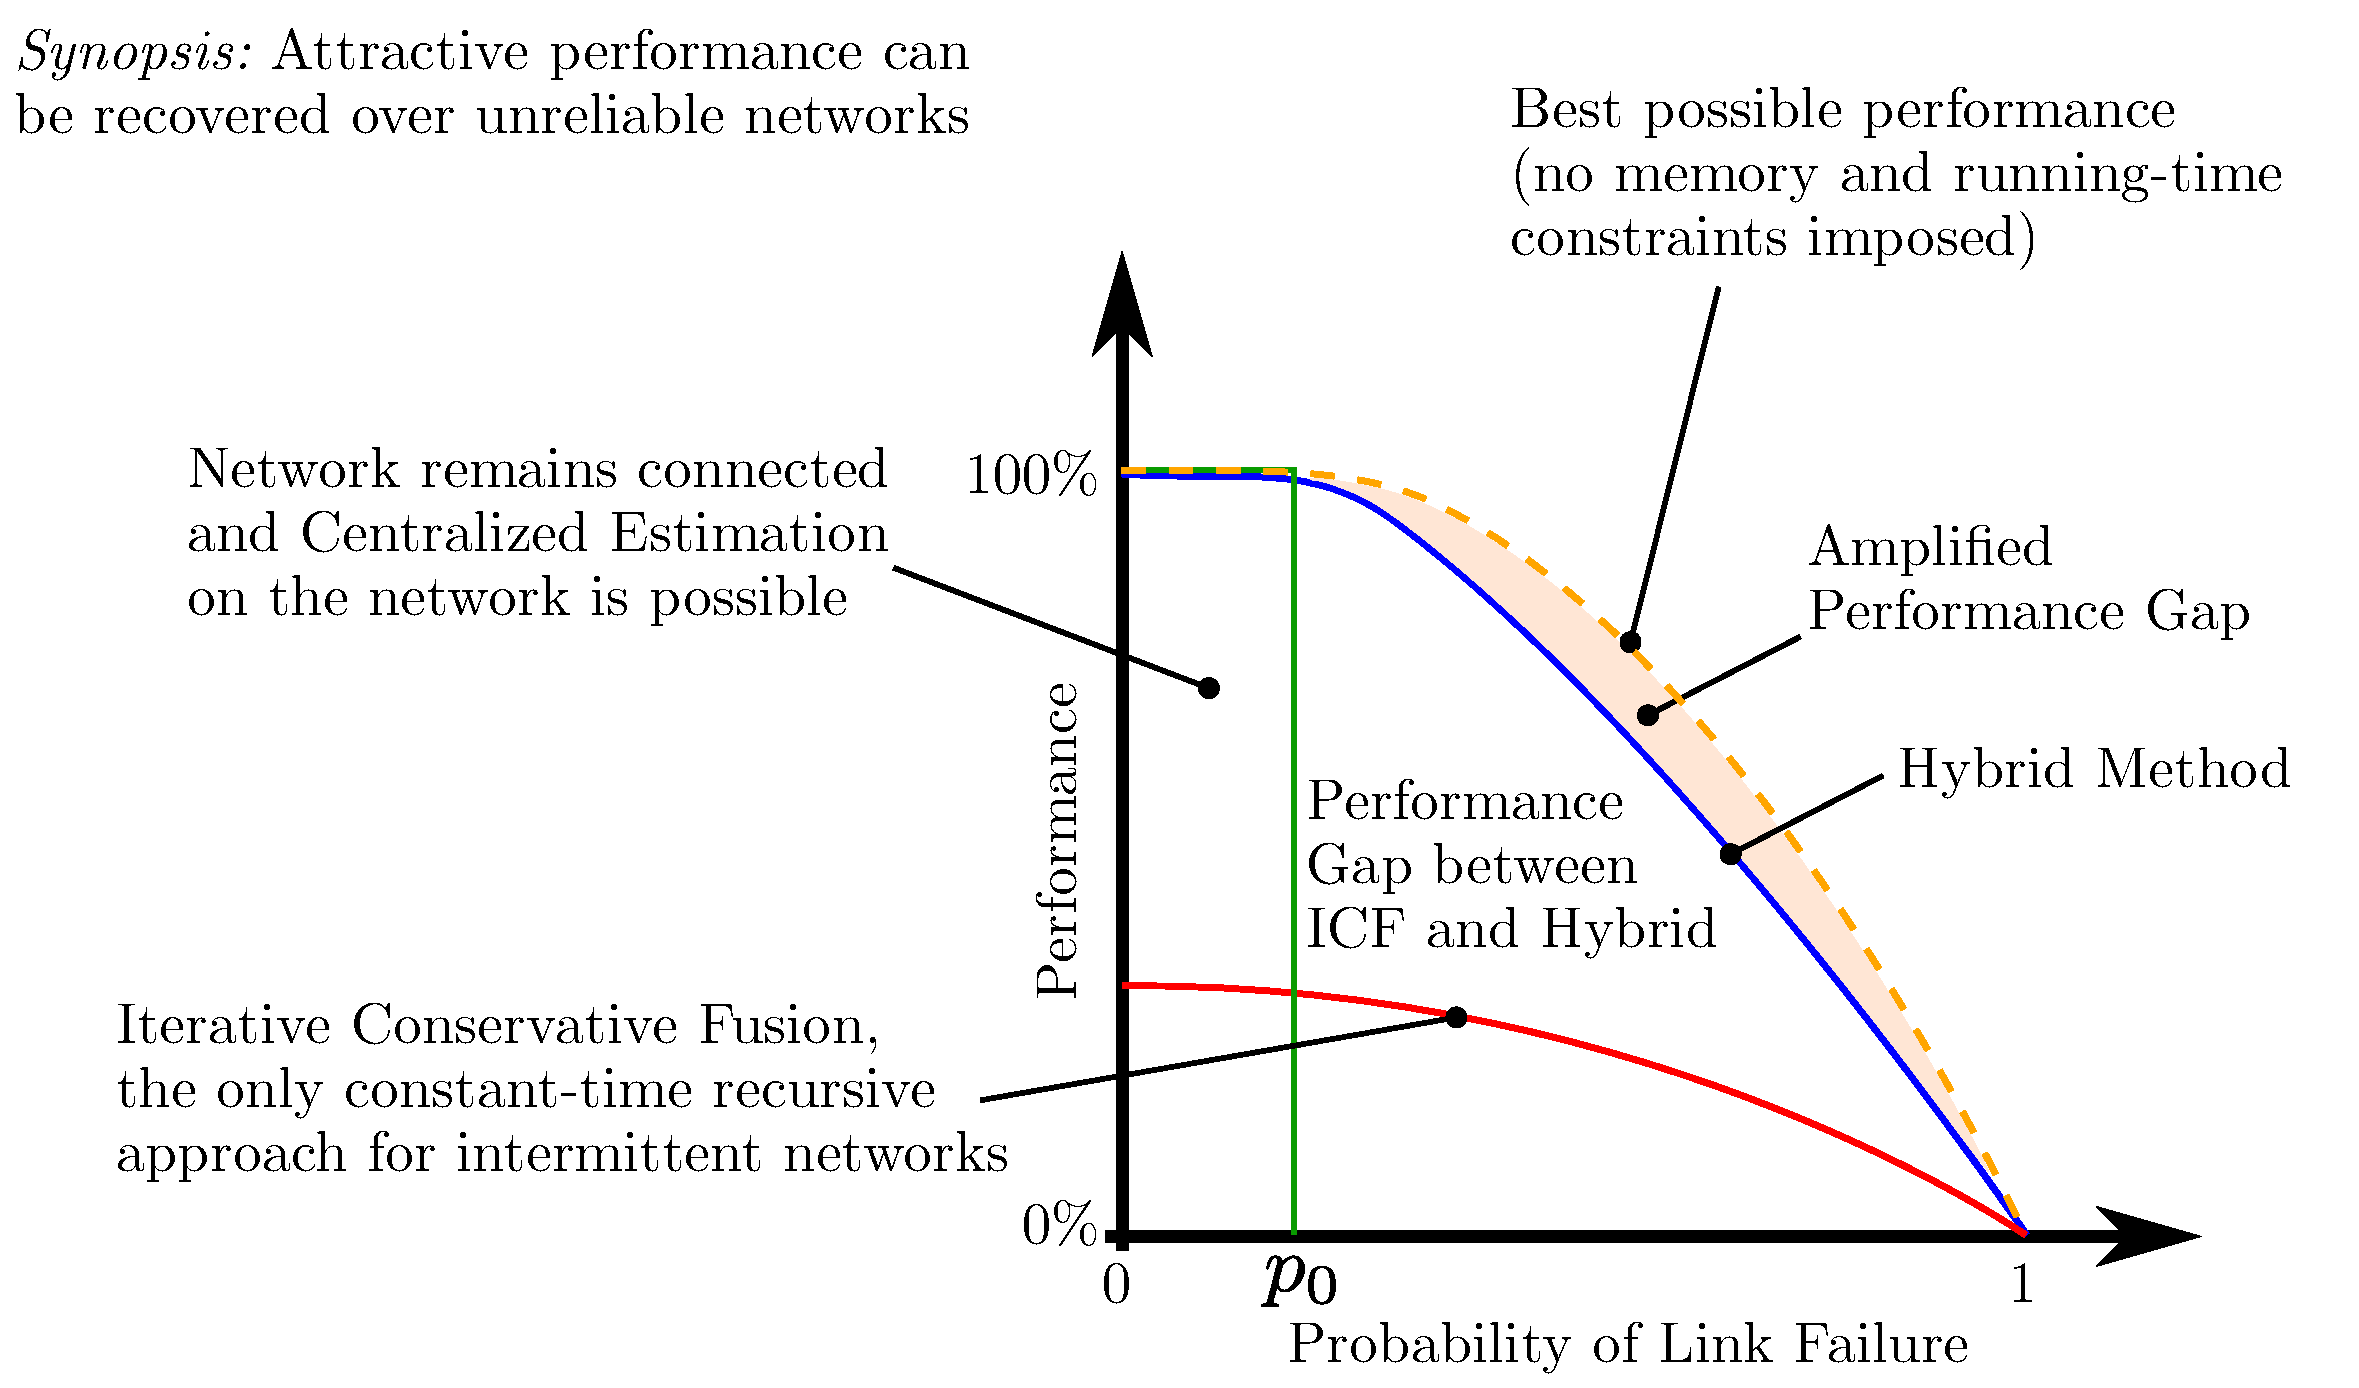
\includegraphics[width=1.0\columnwidth]{./synopsis_for_journal_inkscape_text_black.pdf}
\caption{The synopsis of the paper shown graphically. A centralized method can produce
the highest quality estimates possible, but can only be used when the network
remains fully connected for all time. 
In contrast, Iterative Conservative Fusion (a constant time recursive
approach) is practicable with intermittent connectivity, but its 
conservative nature means that information is diluted, degrading estimation
performance. The method described herein is a hybrid of both, realizing the
``best of both worlds'' in that it achieves excellent performance across a wide range
of network conditions, including recovering centralized performance in the
connected regime.
\label{fig:synopsis} }
\end{figure} 



Figure~\ref{fig:synopsis} shows different estimation methods and illustrates
how the proposed Hybrid method can be situated.  The horizontal axis in the
diagram is the probability of link failure: $p=0$ means that when two agents
that try to establish a communication link will always succeed and $p=1$ means
they will always fail. The vertical axis represents a performance measure, yet
to be defined, that quantifies the similarity of the estimated PMF to the PMF
of an omniscient estimator with access to all observations made by nodes independent from
network topology.  When the network is connected, this is equivalent to the
centralized estimator.  However, there is a threshold $p_0$ (which may in general
depend on the network topology) beyond which the centralized estimator cannot
operate.  Once that threshold has been crossed, the network will likely have
more than one connected component and such components will change over time.
This is the area where the proposed method has unmistakable superiority over
competitors. The threshold $p_0$ may be small for simple network topologies
resulting in a large area that corresponds to DSE under connections of
intermittent connectivity.

Note that in the event of intermittent network disconnection, the estimator
performance will inevitably fall below the omniscient estimator. Even if no
memory and computational limit is imposed and nodes are allowed to keep the
full history of their observations and share such a history with other path
connected nodes on the network, there is always an upper band on the proximity
measure. We show that our method's performance approaches the upper bound,
resulting in a large performance improvement compared with ICF.  

The remainder of the paper is organized as follows.  In
Section~\ref{subsec:assump_not}, the notation used in this paper is explained.
The section also identifies the assumptions and describes the system model.
Section~\ref{subsec:Preliminaries} gives some preliminaries on distributed
state estimation, paving the way for the presentation of the new Hybrid method.
The method itself is presented in Section~\ref{subsec:Method} and, finally, we
evaluate its performance in Section~\ref{sec:experiments}.   

\section{Notation and Model} \label{subsec:assump_not}

\subsection{The Network Topology} 

Assume that we have $n$ homogeneous agents associated with the nodes of a 
graph. These agents can communicate with one another under a time-varying 
undirected network topology $ G_{k} = \langle \mathcal{V},\mathcal{E}_k\rangle 
$ where $\mathcal{V}$ and $\mathcal{E}_k$ are, respectively, the set of graph nodes and edges 
at step $k$. The node corresponding to the $i^\text{th}$ agent is 
denoted by $v_i$. 
If agents $i$ and 
$j$ can communicate directly at step $k$ then
$(v_i,v_j)\in \mathcal{E}_k$. 
The set $\overline{\mathcal{N}}_i$ 
represent 
neighbors of node ${v}_i$ that are connected by an edge to $v_i$. The set 
$\mathcal{N}_i=\overline{\mathcal{N}}_i\cup \{v_i\}$ will also be used in some 
of the equations. The set $\textsc{cc}_k^i$ represents the set of agents 
that are \textit{path-connected} to agent $i$ at step $k$ (the mnemonic being \underline{\sc{c}}onnected \underline{\sc{c}}omponent).

For a time-varying network, there exist connected component sets (or, more briefly, components) that persist over time. 
By this we mean that the subset of nodes comprising the component remains constant, though the internal topology of the graph within the component may vary. 
A component can be uniquely identified by its members, the time of its formation, and its lifetime, i.e., the duration that the set of nodes remains unchanged. Then, at time step $k$, a network $\net_k$ can be represented by a set of components paired with their formation times:
\begin{equation}
	\net_k = {(\textsc{cc}^1,t_{\textsc{cc}^1}), \dots, (\textsc{cc}^M,t_{\textsc{cc}^M})},\quad M<|\mathcal{V}|.
\end{equation}

Robot~$i$ is said to be part of a component $\textsc{cc}^m$  if $v_i\in \textsc{cc}^m$, where the $m$ is used to denote 
an entry from the pairs in $\net_k$, this being an extrinsic view.
We will also find it  convenient to talk of robot~$i$ being
part of component $\textsc{cc}_k^j$, again simply meaning $v_i\in \textsc{cc}_k^j$. 
This latter notation refers to the same component (as robot~$i$ is only in one component at time~$k$) but it emphasizes a component associated with an individual node, in this particular case, stating that robot~$i$ is connected (via some path) to robot~$j$.

The set $T_{cc}=\{t_0, t_1, \dots \}$ contains the timestamps in which a change occurs in the composition of $\net_k$. Additionally, let $t_{c,k} = t_{k+1} - t_{k}$ denote the duration for which all network components comprising $\net_k$ persist. Note that the lifetime of a single component in $\net_k$ can be greater than $t_{c,k}$ if it was formed before $t_{k}$ or if it continues to exist beyond $t_{k+1}$.


For an arbitrary set 
with 
members $\mathbf{b}=\{b_{i_1},\cdots,b_{i_s}\}$, 
the index set $\boldsymbol{I}_{b}=\{i_1,\cdots,i_{s}\}$ contains the indices of
$\mathbf{b}$'s members (and $s\in \mathbb{N} $). We will use the abbreviated
form  $ \bIn = 
\{1,2,\cdots,n\},$ and $\bIk = \{1,2,\cdots,k\}$ to index the agents and time 
steps, respectively.

\subsection{System Model} 

Consider a finite state HMM specified as follows:

\begin{itemize}
\item The HMM has $n_s$ possible states 
 \mbox{$\mathcal{X} = \{S_1,\cdots,S_{n_s}\}$} and also, there are $n_z$ possible observation symbols 
 \mbox{$\mathcal{Z} = \{O_1,\cdots,O_{n_z}\}$}.
\item The random variables $\vect{X}_k \in \mathcal{X}$ and $\vect{Z}_k^i \in
 \mathcal{Z}$ represent the state and observation made by agent $i$ at step $k$,
 respectively. The realizations of those random variables at step $k$ are
 denoted $\vect{x}_k$ and $\vect{z}_k^i$.    
\item The transition model is an $n_s\times n_s$ matrix written
 $\mathcal{P}_{k \vert k-1}\triangleq \pr(\vect{X}_{k} | \XX[]{k-1}{})$. All the
 agents possess this model.
\item Each agent has an observation model, which is an $n_s\times n_z$ 
 matrix written as $\pr(\vect{Z}_{k}^{i} | \vect{X}_{k}), i\in\bIn$. The 
 observation models of different agents may differ.
\item The prior, prediction, and posterior probabilities are $1\times n_s$ random vectors
 \begin{align}
 \pi_{k-1}&\triangleq \pr\left(\XX[]{k-1}{}|\{\zz{k}{i}\}^{i\in\bIn}_{k\in\bIkk}\right),\nonumber\\
 \tilde{\pi}_{k}&\triangleq \pr\left(\XX[]{k}{}|\{\zz{k}{i}\}^{i\in\bIn}_{k\in\bIkk},\XX[]{k-1}{}\right),\nonumber\\
 \pi_{k}&\triangleq \pr\left(\XX[]{k}{}|\{\zz{k}{i}\}^{i\in\bIn}_{k\in\bIk}\right),\nonumber
 \end{align}
 respectively.
\end{itemize}

The above HMM is a well-defined and useful description for many distributed
estimation applications including ones with dynamic state and time-varying
observation models. For example, the following transition and observation
models can be represented in the above form:
\begin{align}
\XX[]{k+1}{} &= f(\XX[]{k+1}{},\ais{\vect{w}}{k}{})\quad \ais{\vect{w}}{k}{} \sim \pr(\ais{\vect{W}}{k}{}), \\
\ZZ{k+1}{i} &= h^i(\XX[]{k+1}{},\ais{\vect{v}}{k}{})\quad \ais{\vect{v}}{k}{} \sim \pr(\ais{\vect{V}}{k}{}), 
\end{align}
in which, $\ais{\vect{W}}{k}{}$ and $\ais{\vect{V}}{k}{}$ are random variables
representing dynamics and observation noise. 

Further, we assume that each agent
has a processor and a sensor on-board. Sensors make observations every $\Delta
t$ seconds and the processors and the network can handle calculations based on
message passing among agents every $\delta t$ seconds. We assume that $\delta t
\ll \Delta t$. We also assume that the agents exchange their information over
the communication channel which is free of both delay and error. 
Communication links are assumed to be symmetric.

The specification above can be extended to
include control inputs but they are omitted as they are not the focus this
paper. 

Henceforward, $\{\ZZ{k}{i}\}^{i\in\bIn}_{k\in\bIk}$ is the indexed family of
all the observations made by all the agents up to step $k$. For each
agent $i$, the variable $\vect{R}_{k}^{ij}, j \in \overline{\mathcal{N}}_i $
denotes the information that node $i$ receives from node $j$, its neighbor at
time $k$. The set $\vect{R}_{k}^i$ contains all the information that node $i$
has received from its neighbors up to step $k$ and $\vect{I}_{k}^i =
\vect{R}_{k}^i \cup \vect{Z}_{k}^i$ represents all the information content that
is available to agent~$i$ at time~$k$. (In general, in this paper, the
information in the variable that bears the superscript $i$ is a version local
to the $i^\text{th}$ agent. Moreover, symbol $\eta$ with or without any
sub/superscript is a normalizing constant.)

\section{Distributed State Estimation} \label{subsec:Preliminaries}

In this section we will review some concepts in \textit{Distributed State
 Estimation} that help us better understand the details of the method developed
in the next section. We first define \textit{Recursive State Estimation} in the
context of HMMs. Then, we discuss what is meant by \textit{Centralized
 Estimation} in the context of networked systems, as this notion has 
been used only informally up till now.
We proceed to define a method,
within the Consensus on Likelihoods (CL) class, called \textit{Distributed
 Consensus Based Filtering} that is particular to systems where agents have
identical prior information. Given that network disconnection and early
stopping of the consensus process yields priors among the
agents that are not identical, we review \textit{Conservative Fusion} and its iterative version as a
remedy for such cases. 

In the context of HMMs, Recursive State Estimation is the process of
recursively computing the posterior probability of a random dynamic process
$\XX[]{k}{}$ conditioned on a sequence of measurements
$\{\zz{k}{i}\}^{i\in\bIn}_{k\in\bIk}$. Bayesian recursive filtering, in a
process with the Markov assumption, has the form
\begin{align}
\label{eq:geb}
&\pr(\XX[]{k}{}|\vect{z}_{k})  = \frac{1}{\eta}\pr(\vect{z}_{k}| \XX[]{k}{})\pr(\XX[]{k}{}|\vect{z}_{k-1},\vect{X}_{k-1}) \\
&= \frac{1}{\eta}\prod_{i=1}^{n} \pr(\vect{z}_{k}^i | \XX[]{k}{}) \int \pr(\vect{X}_{k} | \XX[]{k-1}{}) \pr(\XX[]{k-1}{}|\vect{z}_{k-1}) \text{d}\vect{\XX[]{k-1}}.\nonumber 
\end{align}

Recursive estimation in a sensor network setting for an HMM
can be carried out in the following ways:

\subsection{Centralized Estimation}

Centralized Estimation (CE) involves a single distinguished node in the
network that receives observations $\zz{k}{\bIn} \triangleq
\{\zz{k}{i}\}^{i\in\bIn}$ from the rest. The above Bayesian filtering recursion
for step $k$ of a finite state HMM consists of first calculating the prediction
$\tilde{\pi}_{k}$ according to 

\begin{equation}
\label{eq:pred}
\tilde{\pi}_{k} =  \pi_{k-1}\mathcal{P}_{k \vert k-1},
\end{equation}
then updating via
\begin{equation}
\label{eq:update}
{\pi}_{k} = \frac{1}{\eta}\tilde{\pi}_{k} \mathcal{O}_k,
\end{equation}
where $\mathcal{O}_k$ is an $n_s\times n_s$ diagonal matrix of likelihoods, $\pr(\zz{k}{\bIn}| \XX[]{k}{})$.  

\begin{remark}
 Under CE, for a connected component set $\textsc{cc}$ containing $n_{c}$ nodes, 
 the state Probability Mass Function (PMF) at step $k$ and the initial PMF $\pi_{0}$ are
 related by
 \begin{equation}
 {}^{\suf{CE}}{\pi}_{k} = \frac{1}{{\pi}_{0}T_{1:k}^{\suf{CE}}\mathbf{1}_N}\,\,{\pi_{0}}T_{1:k}^{\suf{CE}},\label{CE-UPDATE} 
 \end{equation}
 where  
 \begin{equation}
 {T}_{1:k}^{\suf{CE}} =\mathcal{P}_{1\vert0}\mathcal{O}_{1}\cdots\mathcal{P}_{k\vert k-1}\mathcal{O}_{k}.
 \end{equation}
\end{remark}

\subsection{Consensus on Likelihoods}
Consensus on Likelihoods (CL) is based on the insight that in \eqref{eq:geb}
one can see that if all agents share the same prior information, they will
recover the centralized estimator's performance if they can reach 
consensus over the product of measurement probabilities. Distributed averaging methods
can be applied here as the nodes need to reach a consensus over the $\log$ of
the joint measurement probabilities (log-likelihood), that is,
\begin{equation}
\tilde{l}_k  = \frac{1}{n} \log \prod_{i=1}^{n} \mathcal{O}_k^i  = \frac{1}{n} \sum_{i=1}^{n} \log \mathcal{O}_k^i = \frac{1}{n} \sum_{i=1}^{n} \tilde{l}_k^i.
\end{equation}
Once consensus is reached, the updated estimate is 
\begin{equation}
\label{eq:dlc}
{\pi}_{k}  = \frac{1}{\eta}\overbrace{ \underbrace{{\pi}_{k-1}}_{\text{prior}} 
\mathcal{P}_{k \vert k-1}  
}^{\text{prediction}}\underbrace{e^{n\tilde{l}_k}}_{\text{likelihood}}.
\end{equation}

Coming to some consensus over likelihoods can be achieved for the discrete state variables using a distributed averaging method based on Metropolis-Hastings Markov Chains (MHMC). To avoid confusion we use $m$ to indicate consensus iterations throughout this paper. On a communication graph $G$ one can use a message passing protocol of the form 
\begin{align}
&\vect{\psi}^i(m+1)=\textstyle {\sum\nolimits _{j=1}^{|\mathcal{N}_{i}|}} \gamma_{ij}(m)\vect{\psi}^j(m),\\
& \text{such that } \sum_{m}  \gamma_{ij}(m) = 1,\,\,  \vect{\psi}^i(0)=  \tilde{l}_k^i,\nonumber
\end{align}
to calculate the average of the values.
On the graph nodes in which $d_{i}(m)=|\mathcal{N}^i|$ is the degree of the node $v_i$, 
one sets
\begin{equation}
\label{eq:mhmc}
\gamma_{ij}(m) =
\begin{cases}
{\frac{1}{1+\max\{d_{i}(m),d_{j}(m)\}}}      &  \text{if } (i,j) \in \mathcal{E}_{m}, \\
1-\sum\limits_{{(i,n)} \in \mathcal{E}}\gamma_{in}  &  \text{if } i = j,\\
0 & \text{otherwise}.
\end{cases}
\end{equation}
With this messaging passing protocol $$\lim_{m\rightarrow \infty} \vect{\psi}^i(m) = \tilde{l}_k.$$

Note that for each node $i$, the $\gamma_{ij}$'s depend only on the degrees of
its neighboring nodes. As stated earlier, once consensus has been reached over
likelihoods, the centralized estimate will be recovered. A prerequisite for
this method to work is that the network remains connected, a 
requirement which is too restrictive for many applications.

\begin{remark}
For a connected component set $\textsc{cc}$ containing $n_{c}$ nodes
the CL method's likelihood after consensus is equivalent to the likelihood of collective information of the nodes in $\textsc{cc}$. This means that if the consensus process converges,
Introducing the concise notation 
\begin{equation}
\mathcal{O}_{k}^{{\{\omega_{1:n_{c}}\}}_{k}} = \prod_{j = 1}^{n_{c}}  \big[\mathcal{O}_k^j]^{\omega_{j,k}},
\end{equation} 
we see that, if the consensus process converges,
\begin{equation}
\mathcal{O}_{k}^{{\{n_c\omega_{1:n_{c}}^{\suf{CL}}\}}_{k}}= \mathcal{O}_{k}^{{\{n_c\frac{1}{n_c}\}}_{k}} = \mathcal{O}_{k}.
\label{eq:CL-CONVERGE} 
\end{equation}
Even if the topology of the network changes, as long as the nodes that comprise $\textsc{cc}$ remain unchanged, the state PMF at step $k$ and the initial PMF $\pi_{0}$ are related by
\begin{equation}
{}^{\suf{CL}}{\pi}_{k} = \frac{1}{{\pi}_{0}T_{1:k}^{\suf{CL}}\mathbf{1}_N}\,\,{\pi_{0}}T_{1:k}^{\suf{CL}} 
,\label{CL-UPDATE} 
\end{equation}
where  
\begin{equation}
\label{CL-INC}
{T}_{1:k}^{\suf{CL}}  =\mathcal{P}_{1\vert0}\mathcal{O}_{1}^{{\{n_c\omega_{1:n_{c}}^{\suf{CL}}\}}_{1}}\cdots\mathcal{P}_{k\vert k-1}\mathcal{O}_{k}^{{\{n_c\omega_{1:n_{c}}^{\suf{CL}}\}}_{k}}. 
\end{equation}
The expression in~\eqref{eq:CL-CONVERGE} guarantees that after convergence,
from the same initial condition, the posterior of CL is equal to
\emph{CE} and 
\begin{equation} \label{TCL}
{T}_{1:k}^{\suf{CE}} = {T}_{1:k}^{\suf{CL}}  =\mathcal{P}_{1\vert0}\mathcal{O}_{1}\cdots\mathcal{P}_{k\vert k-1}\mathcal{O}_{k}.
\end{equation}
The formal requirement for the above expression to hold is that the consensus
process converges with a network dependent rate $\sigma_{\textsc{cc}}$ and, for
$\delta t$ and $\Delta t$ defined as before, $\sigma_{\textsc{cc}}\delta t \ll
\Delta t$.
\end{remark}

Success of this method is contingent upon node priors being equal. Next,
we discuss the conventional method employed for cases with
node priors that are not equal.

\subsection{Iterative Conservative Filtering} 

Iterative Conservative Filtering  (ICF) is an approach where, instead of
putting effort into ascertaining the dependencies between agents' information,
a fusion rule is designed to guarantee that no double counting of mutual
information can occur.  This usually results in the replacement of independent
information with some form of approximation which is conservative.  Such a
treatment dilutes the information available from observations, resulting in
performance that is inferior to distributed filters which do not suffer the
degradation introduced by this approximation.

Since, in general, \emph{Conservative Approximate Distributed Filtering} relies
on fusion rules that combine conservative approximation of local PMFs, we need
to clarify what constitutes a conservative approximation for a PMF. 
Mechanisms of conservative fusion follow straightforwardly thereafter. 

Conservative approximation of a PMF is only possible under certain conditions.
Bailey, Julier, and Agamennoni~\cite{bailey2012conservative} introduced a set of
sufficient conditions for a PMF, $\tilde{\pr}(\vect{X})$, to satisfy in order to
be deemed a conservative approximation of a second PMF, $\pr(\vect{X})$. The
conditions are:
\begin{description}
\item [(P1)] The property of non-decreasing entropy:
$$\begin{aligned}
\text{H}(\pr(\vect{X})) \leq \text{H}(\tilde{\pr}(\vect{X}));
\end{aligned}$$
\item [(P2)] The order preservation property: 
$$\begin{aligned}
\pr(\vect{x}_i) \leq \pr(\vect{x}_j) \ \text{iff}\  \tilde{\pr}(\vect{x}_i) \leq \tilde{\pr}(\vect{x}_j), \,\, \forall \vect{x}_i,\vect{x}_j\in\vect{X}.
 \end{aligned}$$
\end{description}

Then Conservative Fusion (CF) of two PMFs can be achieved for two probability
distribution functions $\pr_a(\vect{X | \vect{I}_a})$ and $\pr_b(\vect{X} |
\vect{I}_b)$, with the \emph{Geometric Mean Density Rule (GMD)}:
\begin{equation}
\begin{aligned}
\pr_c(\vect{X})&= \frac{1}{\eta_c} \pr_a(\vect{X| \vect{I}_a})^\omega \pr_b(\vect{X| \vect{I}_b})^{1-\omega}\\
=& \frac{1}{\eta_c} \pr_a(\vect{X| \vect{I}_a} \setminus \vect{I}_b)^\omega \pr_b(\vect{X| \vect{I}_b} \setminus \vect{I}_b)^{1-\omega} \pr_a(\vect{X| \vect{I}_a} \cap \vect{I}_b),\\
\end{aligned}
\end{equation}  
in which, $0\leq\omega\leq1$. 
Note that in the above equation the PMFs are raised to the power of $\omega$
and multiplied together element-wise. This rule never double counts mutual
information, replacing independent components with a conservative
approximation. The interesting property of this fusion rule is that it works
without the knowledge of the dependence of the two initial PMFs. This  rule can
also be generalized to more than two PMFs. For example, in the context of this
paper, node~$i$ calculates a conservative approximation of the centralized
estimate and stores it in $\tilde{\pi}^i$. The GMD fusion of these estimates is
also a conservative approximation of the centralized estimate. 
\begin{equation}
\label{eq:CFb}
\tilde{\pi}_{k} =\frac{1}{\eta} \prod_{i=1}^{n} {(\tilde{\pi}_{k}^i)}^{\omega_i},\text{ such that } \quad \textstyle {\sum\nolimits_{i=1}^{n} \omega_i=1}.
\end{equation}

\begin{remark}
 Several criteria have been proposed to choose the $\omega_i$. One such
 criterion is~\cite{ajgl2015design}:
 \begin{equation}
 \label{eq:crit}
 \tilde{\pi}=\arg\min_{\pi}\max_i\{\mathcal{D}(\pi\Vert \tilde{\pi}^{i})\}, \end{equation}
 where the $\mathcal{D}(\pi\Vert \tilde{\pi}^{i})$ is the Kullback-Leibler divergence between $\pi$ and $\tilde{\pi}^i$.
\end{remark}

\begin{remark}
 It is shown in~\cite{bailey2012conservative} that raising a PMF to the power of
 $\omega \leq 1$ reduces its entropy. From \eqref{eq:CFb} it can be seen that
 applying the GMD rule reduces the entropy of the likelihood probabilities that
 are independent. In general, doing so is undesirable 
 and the likelihood probabilities can be treated separately to 
 avoid this.
\end{remark}

    \emph{Iterative CF (ICF)} is achieved as follows. At the first 
    iteration of consensus, $m=0$, for each agent $j$, take the current local 
    estimate ${\pi}_{k-1}^j$ and calculate the prediction $\tilde{\pi}_k^j$. 
    Initialize the local 
    consensus variable to be  $$\mathcal{\phi}^j(0) 
    =\frac{1}{\eta_i}\tilde{\pi}_k^j\mathcal{O}_k^j. $$ 

Let $\vect{\omega}= \{\omega_{j}\}^{j\in\bIs{{\cal N}^{i}(m)}}$ and find 
$\vect{\omega}^*$ such 
that 
\begin{equation}
\label{eq:opt_problem}
\begin{aligned}
\vect{\omega}^* &= { \arg \min_{\omega}}  \mathcal{J} \big( \frac{1}{\eta} {\prod_{j \in {\cal N}^{i}(m)} }  \big[\mathcal{\phi}^j(m)\big]^{\omega_{j}} \big), \\
\text{such that }&  {\sum_{j \in {\cal N}^{i}(m)}} \omega_{j}= 1 \text{ and }\omega_j\geq 0, \quad \forall j,
\end{aligned}
\end{equation}
where $\eta$ is the normalization constant and $\mathcal{J}(\cdot)$ is an 
optimization objective function. Specifically, it can be entropy $H(\cdot)$ or 
the criterion in \eqref{eq:crit}. The $\mathcal{\phi}^i$s are then updated locally 
for the next consensus iteration with
\begin{equation}
\mathcal{\phi}^i(m + 1) =  \frac{1}{\eta^*} {\prod\nolimits_{j \in {\cal N}^{i}(m)} }  \big[\mathcal{\phi}^j(m)\big]^{\omega_{j}^*}.
\end{equation}
It is straightforward to show that after repeating this process, 
for all $j \in \textsc{cc}^i_k$, the local variables $\mathcal{\phi}^j(m)$ converge 
to a unique $\mathcal{\phi}^*$. Moreover, $\mathcal{\phi}^*$ is
a convex combination of initial consensus 
variables of all the agents in the set $\textsc{cc}^i_k$, that is,
for all $ i \in \textsc{cc}^i_k$,
\begin{align}
\lim\limits_{m\rightarrow 
\infty}\vect{\phi}^{i}(m) = \mathcal{\phi}^*&= 
\frac{1}{\eta} 
{\prod\nolimits_{j \in \bIs{\suf{cc}^i_k} } }  
\big[\mathcal{\phi}^j(0)\big]^{\omega_{j}^*}\\
&= \frac{1}{\eta}{\prod\nolimits_{j \in \bIs{\suf{cc}^i_k} } }\big[{\pi}_{k-1}^j\mathcal{P}_{k\vert k-1}\mathcal{O}_k^j\big]^{\omega_{j}^*}.
\end{align}
To repeat the process iteratively, set ${\pi}_{k+1}^j = \mathcal{\phi}^*, \forall j \in \textsc{cc}^i_k$ and 
repeat the whole process for step $k+1$.

\begin{remark}
For a connected component \textsc{cc} containing $n_{c}$ nodes, once
the consensus process has converged, we can write the one step estimate update
as 
\begin{align}
\label{eq:cf-recur}
{}^{\suf{ICF}}{\pi}_{k} &= \tau\big({}^{\suf{ICF}}{\pi}_{k-1}\big) \nonumber\\
&= \frac{1}{\eta}\prod_{j = 1}^{n_{c}}  \big[{}^{\suf{ICF}}{\pi}_{k-1}\mathcal{P}_{k\vert k-1}\mathcal{O}_k^j\big]^{\omega_{j,k}}.
\end{align} 

The expression relating initial PMF and state PMF at step~$k$, unlike previous methods, is a nested expression
\begin{equation}
\label{eq:icfprop}
{}^{\suf{ICF}}{\pi}_{k} = \tau^k\big({\pi}_{0}\big)=\tau\big(\tau\big(\cdots\tau\big({\pi}_{0}\big)\cdots\big)\big). \\
\end{equation}
% I removed the ICF from \pi_0; that is because the previous instances CE + CL didn't have that to denote the PMF. I considered adding them there, but they're actually using the overall prior --- what their \pi_0 is doesn't depend on the choice of method.
This shows that under general conditions, even with the same initial PMF,
the ICF method will not generate the same estimate as CE or CL do over
time. The only exception is the trivial case of a fully disconnected network
where, of course, all methods become equivalent.
\end{remark}

\begin{remark}
In ICF the nodes' priors are allowed to be different. For the \textsc{cc} 
described in the previous remark, it only takes one consensus process for all
the nodes to have the same prior and be able to update their state using
\eqref{eq:cf-recur}. For a connected set an alternative can be considered:
one can use ICF on the priors and, once consensus has been reached, use CL to
update the state PMF. This is equivalent to first calculating  

\begin{equation}
{}^{\suf{ICF}}\bar{\pi}_{0} = \frac{1}{\eta}\prod_{j = 1}^{n_{c}}  \big[{}^{\suf{ICF}}{\pi}^j_{0}\big]^{\omega_{j,0}}, 
\end{equation} 
and then using \eqref{CL-UPDATE} and \eqref{CL-INC} with $\pi_0 =
{}^{\suf{ICF}}\bar{\pi}_{0}$. The striking benefit is that we can 
recover the posterior of CE. 
\end{remark}

In the previous remark we illustrated how mixing ICF and CL could be beneficial
for a connected set of nodes with priors that differ.  This is the first
indication of the potential for some hybrid between ICF and CL that would be
especially useful for networks with intermittent connections, where connected
components change over time and it is necessary to handle
unequal priors repeatedly.  The next section describes such a method.  Under the
connectivity constraints just mentioned (intermittent communication with
connected components that churn) we are able to show that when the lifetime of
the connected components in the network is long enough, one can asymptotically
recover CE's performance.

\section{Hybrid ICF and CL} 
\label{subsec:Method}

We propose a Hybrid approach that uses ICF to reach consensus over priors and 
the CL
%Distributed Consensus Based Filtering method (outlined above, which we refer to as CL hereafter) 
for distributed averaging of local information updates. Our method is
presented in detail as pseudo-code in Algorithm~\ref{alg:inf-predict}. 

To give a meaningful interpretation, imagine a 
scenario consisting of $n$ agents observing $\vect{x}_k$, the state of a 
Markov chain at time $k$, and communicating with each other through a 
time-varying network topology. Initially the agents start with  priors 
$\{{\pi}_0^i\}^{i \in \bIn} $. At step $k$ the chain transitions to the new 
state $\vect{x}_k$ and the agents calculate their own local prediction 
$\{\tilde{{\pi}}_k^i\}^{i \in \bIn} $ (line~\ref{alg:localpred} in the algorithm). 
They then make 
observations $\{\vect{z}_k^i\}^{i \in \bIn}$, and compute the local likelihood  
matrices $\{\mathcal{O}_k^i\}^{i \in \bIn}$ (line~\ref{alg:localobs} in the algorithm).

In the rest of the algorithm, the ICF approach is used to reach 
consensus over the priors using \eqref{eq:opt_problem} recursively. The CL 
approach is used to reach consensus over the new information available to 
agent $i$ from other agents that it is path-connected to, i.e., 
$\textstyle \sum_{{j \in \bIs{\suf{cc}^i_k} }}  \tilde{l}_k^i$. In line~\ref{alg:posterior} of the algorithm, $|\textsc{cc}^i_k|$ is the number of agents that form a 
connected 
component with agent~$i$, and can be determined by assigning unique IDs to the 
agents and 
passing these IDs along with the consensus variables. Each agent keeps track of 
the unique IDs it receives, passing them to its neighbors.

\begin{algorithm}[!ht]
\SetKwInOut{Input}{Input}
\Input{${\pi}^i_{k-1}$ }
\hrule
\caption{Hybrid Method}
\label{alg:inf-predict}
Use \eqref{eq:update} to calculate  $\tilde{\pi}^i_{k}$\label{alg:localpred}
%$[{y}_j^-(t_0) ,{Y}_j^-(t_0)] =\textsc{Pred}[{y}_j(t_0),{Y}_j(t_0)]$ 

Collect local observation ${z}^i_{k}$ and calculate ${\mathcal{O}}^i_{k}$ 
and $\tilde{l}_k^i$\label{alg:localobs}

Initialize consensus variables:
\begin{equation*}
\YY[]{0}{i} = \tilde{\pi}^i_{k}, \quad \yy[]{0}{i} = \tilde{l}_k^i
\end{equation*}

$m=0$\\
\While{\text{not converged}} 
{ $\textsc{Broadcast}[ \yy[]{m}{i}, \YY[]{m}{i}]$\\
$\textsc{Receive}[ \yy[]{m}{j}, \YY[]{m}{j} ] \quad \forall j \in 
\mathcal{N}^i$\\ 
Collect received data 
\begin{equation*}
\mathcal{C}^i(m)=\{  \YY[]{m}{j \in  \mathcal{N}^i} \}, \quad  
\mathcal{M}^i(m)=\{  \yy[]{m}{j \in  \mathcal{N}^i} \}.
\end{equation*}

Do one iteration of ICF on consensus variables for local prior 
information $\mathcal{C}^i_m$:
$$ \YY[]{m+1}{i}=\textsc{icf}\left[\mathcal{C}^i(m)\right].$$\\
Do one iteration of MHMC on consensus variables for new 
information:   $$ \yy[]{m+1}{i}=\textsc{mhmc}\left[\mathcal{M}^i(m)\right].$$\\
$m\leftarrow m+1$\\
}
Calculate posteriors according to:\label{alg:posterior}
\begin{equation*}\textbf{}
{\pi}^i_{k} = e^{|\textsc{cc}^i_k|\yy[]{m}{i}}\YY[]{m}{i}.
\end{equation*}
\hrule\vspace*{4pt}
\end{algorithm}

\subsection{Performance Analysis}
\label{subsec:hyb_analysis}

To understand the performance of the Hybrid method, we introduce an estimator
variant that, though impractical in itself,
serves as a useful benchmark for comparison. We use it to conduct an analysis
of the comparative performance of the ICF and Hybrid methods. 

As was illustrated in Figure~\ref{fig:synopsis}, beyond a certain point,
degradation of the network connectivity causes a catastrophic failure of a
centralized estimator.  If one wishes to analyze the performance of an
estimator by comparing its efficiency to an ideal estimator, this poses a
dilemma.  Comparing against the
centralized estimator can hardly be deemed to be meaningful when it
must be granted the ability to fuse observations that
are inaccessible to a decentralized estimator (e.g., owing to observations
being on the opposite side of a network partition). Doing so causes
performance measures to be skewed by the unavailability of data rather than the 
actual estimation process itself.

This motivates consideration of an estimator with performance that is more
realistic.  As will become apparent shortly, a \emph{Full History Sharing Estimator (FHS)} (outlined below) incorporates all the information possible while respecting
network topology constraints and, thus, constitutes the proper upper limit for
estimator performance.

Under FHS, at each step $k$, every agent $i$ has access to the full history of
observations of all the agents that it is path connected to at the current
step.  Then ${}^{\suf{FHS}}{\pi}_{k}$ is obtained by going back to the initial
step, $k=0$, and updating the state PMF sequentially.  The update at each step
uses all the available observations drawn from the full history. Obviously
such calculations quickly become infeasible, but we ignore the computational
complexity and only use ${}^{\suf{FHS}}{\pi}_{k}$ to establish a reference
performance.  Note that under FHS, even though the whole PMF history is
recalculated at each step, the comparison between ${}^{\suf{FHS}}{\pi}_{k}$ and
alternative estimates only involves the PMF at the current point in time.

For our theoretical analysis, we focus on periods of time where the connected
components in the network remain unchanged. Note that this assumption allows
for change in the network topology so long as it does not result in any change in the
connected component sets $\textsc{cc}_k$. We also make the assumption that
consensus processes, of any type, run for enough time to converge for every
estimation step.

With these assumptions, the expression relating ${}^{\suf{FHS}}{\pi}_{k+1}$ and
the initial PMF, ${\pi}_{0}$, is 

\begin{equation}
{}^{\suf{FHS}}{\pi}_{k+1} = \frac{1}{{\pi}_{0}T_{1:k}^{\suf{FHS}}\mathbf{1}_N}\,\,{\pi_{0}}T_{1:k}^{\suf{FHS}},\label{FHS-UPDATE}
\end{equation}
where  
\begin{equation}\label{TFHS}
{T}_{1:k}^{\suf{FHS}}=\mathcal{P}_{1\vert0}\mathcal{O}_{1}\cdots\mathcal{P}_{k\vert k-1}\mathcal{O}_{k}.
\end{equation}

\begin{lemma}
\label{lemma:l1convergence}
Consider the Distributed State Estimation problem of a HMM with a time-varying
network topology $G_{k} = \langle \mathcal{V},\mathcal{E}_k\rangle$ as
described in Section~\ref{subsec:assump_not}. At time $k_0$ let $\textsc{cc}^m$
be the $m^\text{th}$ connected component containing $|\textsc{cc}^m|=n_m$ nodes.
Further assume that $\textsc{cc}^m$ remains unchanged for the next $k$ steps.
Then, during the time $k_0 \leq t\leq k_0+k$, and for all the nodes in
$\textsc{cc}^m$, the Hybrid estimator converges at a geometric rate to the FHS
estimator, when the following conditions are satisfied:

\begin{itemize}
\item The consensus process converges with a network dependent rate
$\sigma_{{\textsc{cc}^m}}$ and for $\delta t$, the consensus update rate, and
$\Delta t$, the time interval between consecutive observations, we have
$\sigma_{{\textsc{cc}^m}}\delta t \ll \Delta t$. 

\item The resultant matrix product of the pairs
$H(t)\triangleq\mathcal{P}_{t\vert t-1}\mathcal{O}_{t}$ is an allowable
non-negative matrix, i.e., each row and column of $H(t)$ has at least one
positive element. 

\item For a fixed $t_0\geq k_0$, all the elements of the product chains of both
estimators are strictly positive, i.e. ${T}_{k_0:t_0}^{\suf{FHS}}>0$ and
${T}_{k_0:t_0}^{\suf{HYB}}>0$.

\item For a fixed $\gamma$, independent of $t$,
\begin{equation}
\frac{\underset{i,j}{\min}^+ h_{i,j}(t)}{\underset{i,j}{\max}\; h_{i,j}(t)}\geq\gamma >0,
\end{equation}
where, $h_{i,j}(t)$ is the $(i,j)$ element of $H(t)\triangleq\mathcal{P}_{t\vert t-1}\mathcal{O}_{t}$,  and $\min^+$ is the minimum over the positive elements.
\end{itemize}
\end{lemma}
\begin{proof}
We have already established the main part of the proof by showing that, if the
consensus process converges, the inhomogeneous chain of matrix products in
\eqref{TCL} and \eqref{TFHS} for a connected component are identical. 
Full history sharing among agents results in a common prior
for $\textsc{cc}^m$ as ${}^\suf{FHS}\pi_{{\textsc{cc}^m},k_0}$. Under the Hybrid method the
agents perform conservative fusion of their priors which converges to a unique
prior denoted as ${}^\suf{HYB}\pi_{{\textsc{cc}^m},k_0}$. The priors for the two estimators
are not the same in general. However, from the moment of connection onwards, as
long as $\textsc{cc}^m$ remains unchanged, the inhomogeneous chain of matrix
products
that results in posterior estimates is equivalent for both methods as shown
by \eqref{TCL} and \eqref{TFHS}, specifically\\ $${T}_{k_0:k}^*  \triangleq
{T}_{k_0:k}^{\suf{FHS}}={T}_{k_0:k}^{\suf{HYB}}.$$ Hence, based on Theorem~3.3
of~\cite{seneta2006non}, for which the last three conditions given are required,
${T}_{k_0:k}^*$ converges to a rank~1 matrix, which consequently renders the
initial priors ${}^\suf{FHS}\pi_{{\textsc{cc}^m},k_0}$, and ${}^\suf{HYB}\pi_{{\textsc{cc}^m},k_0}$
irrelevant. Therefore, the posterior of both estimators converge to the same
stationary distribution of ${T}_{k_0:k}^*$ and, furthermore, they do so at a geometric rate.
\end{proof}

\begin{remark}
\label{rem:ergodicity}
The convergence of ${T}_{k_0:k}^*$ to a rank~1 matrix is termed weak
ergodicity~\cite{seneta2006non,anderson1997forgetting}. Moreover, one can use
the results of~\cite{liverani1999probabilistic} to show 
that there exists some $\rho_{t_0} < 1$ and $ r_{t_0}\le \infty$ so that  
the decay of the $L^1$ norm between the
posteriors of the two methods is bounded by
$$\left\|{}^\suf{FHS}\pi^j_{t_0} {T}_{t_0:t_0+n}^* - {}^\suf{HYB}\pi^j_{t_0} {T}_{t_0:t_0+n}^* \right\|_1 \leq r_{t_0}\rho_{t_0}^{n}.$$ 
The above expression is the basis for the next lemma. 
It is also worth pointing out that the geometric nature of this convergence is clearly visible in the
plots showing the method's empirical performance, as  presented in the following section.
\end{remark}

The analysis so far shows that the formation of connected components, and their lifetime, plays an important role in the performance of DSEs. 
This, in addition to the weak ergodicity property of ${T}_{k_0:k}^*$, provides practical insight for system designers. 
One can link the lifetime of a component to $L^1$ convergence of Hybrid's PMF to FHS's estimates. 
Also, one might establish some other performance measure for estimate quality and wish to know the requirements on $t_{c,k}$ needed to ensure that the gap between FHS and Hybrid average performance over time is smaller than some desired tolerance. 
In order to examine these design choices, we need the following definitions.

Let $\mathcal{C}(\cdot)$ be a Lipschitz continuous performance metric that assigns a scalar to a PMF. By definition
\begin{equation}
	\|\mathcal{C}(\pi_1)-\mathcal{C}(\pi_2)\|_1, \le L\|\pi_1-\pi_2\|_1
\end{equation} 
where $L$ is the Lipschitz constant. 

\begin{lemma}
\label{lem:l1conv}
Let $\textsc{cc}^m$ be a component that was formed at time~$t_0$ and persists for $n$~steps. Let  ${T}_{t_0:t_0 + n}^*$ represent the inhomogeneous chain of matrix
products that describe the FHS and Hybrid methods for this period. Suppose that FHS and Hybrid priors at time~$t_0$ are ${}^\suf{FHS}\pi^j_{t_0}$ and ${}^\suf{HYB}\pi^j_{t_0}$, respectively. 
For any desired convergence, specified via $\epsilon_1$ such that
	\begin{equation}
	\label{eq:l1conv}
	\left\| {}^\suf{FHS}\pi^j_{t_0} T^*_{t_0:t_0+n}  - {}^\suf{HYB}\pi^j_{t_0} T^*_{t_0:t_0+n} \right\|_1 \leq \epsilon_1.
	\end{equation}
	$\textsc{cc}^m$ should persist for at least $n = N_{\epsilon_1}$ steps where
	\begin{equation}
    \label{eq:eps1}
		N_{\epsilon_1}  = (\log_{\rho_{t_0}}\epsilon_1 - \log_{\rho_{t_0}}r_{t_0})
	\end{equation}
	and $\rho_{t_0}$ and $r_{t_0}$ are constants defined in Remark \ref{rem:ergodicity}.
\end{lemma}
The lemma is easily proved by taking the logarithm from both sides of inequality \eqref{eq:l1conv} and using Remark~\ref{rem:ergodicity}.

\begin{prop}
\label{prop:netperf}
Consider the behavior of agent~$j$ over period of time $T$, and its
connected components for that duration $\textsc{cc}^j_{t_0}, \textsc{cc}^j_{t_1}, \dots \textsc{cc}^j_{t_m}$.
Let the average performance measure of agents~$j$ for FHS and Hybrid methods be ${}^\suf{FHS}J^{j}$ and ${}^\suf{HYB}J^{j}$, respectively. For a given $\epsilon_1$  that satisfies \eqref{eq:l1conv} and for a desired $\epsilon_2>L\epsilon_1$ gap between the average performance of FHS and Hybrid so that 
\begin{equation}
\label{eq:prop1eq}
\left\|{}^\suf{FHS}J^{j} - {}^\suf{HYB}J^{j} \right\|_1 \le \epsilon_2,
\end{equation}
the components $\textsc{cc}^j_{t}$, $t \in \{t_0, t_1, \dots, t_m\}$ should persist at least $ N_{\epsilon_2}$ steps, where
\begin{equation}
\label{eq:neps2}
N_{\epsilon_2} = \frac{L N_{\epsilon_1}(2-\epsilon_1)}{(\epsilon_2 - L\epsilon_1)}
\end{equation}
in which $N_{\epsilon_1}$ is calculated based on \eqref{eq:eps1} and $L$ is the Lipschitz constant for function $\mathcal{C(\cdot)}$
\end{prop}

\begin{proof}
By definition, ${}^\suf{FHS}J^{j}$ and ${}^\suf{HYB}J^{j}$ are 
\begin{equation}
{}^\suf{FHS}J^{j} \triangleq  \frac{1}{T} \sum_{t=t_0}^{t_0+T} \mathcal{C}( {}^\suf{FHS}\pi_{t}^{j}), \quad  
{}^\suf{HYB}J^{j} \triangleq  \frac{1}{T} \sum_{t=t_0}^{t_0+T} \mathcal{C}( {}^\suf{HYB}\pi_{t}^{j}).
\end{equation}	
Then we have 
\begin{align}
\left\|{}^\suf{FHS}J^{j} - {}^\suf{HYB}J^{j} \right\|_1&=  \frac{1}{T}\left\|\sum_{t=t_0}^{t_0+T} \mathcal{C}( {}^\suf{FHS}\pi_{t}^{j}) - \mathcal{C}( {}^\suf{HYB}\pi_{t}^{j})\right\|_1 \\
&\le  \frac{1}{T}\sum_{t=t_0}^{t_0+T}\left\| \mathcal{C}( {}^\suf{FHS}\pi_{t}^{j}) - \mathcal{C}( {}^\suf{HYB}\pi_{t}^{j})\right\|_1\\
&\le  \frac{L}{T} \sum_{t=t_0}^{t_0+T}  \left\| {}^\suf{FHS}\pi_{t}^{j} - {}^\suf{HYB}\pi_{t}^{j}\right\|_1.
\end{align}
Now consider that during the time period from $t_{k}$ to $t_{k+1}$ the $j^{\text{th}}$ robot belongs to a connected component whose members are fixed. Then, from  Lemma~\ref{lemma:l1convergence},
for some 
$\rho_{t_k} < 1 $ and some $r_{t_k} < \infty$, we have
\begin{equation}
\left\| 
{}^\suf{FHS}\pi^j_{t_{k}} T^*_{t_{k}:t_{k}+n}  - {}^\suf{HYB}\pi^j_{t_{k}} T^*_{t_{k}:t_{k}+n} 
\right\|_1 \leq r_{t_k} \rho_{t_k} ^ n,
\end{equation}
for all $n \leq t_{k+1} - t_k$.

For the given $\epsilon_1 > 0$, consider all connected components that agent $j$ belongs to in time interval $[t_0,t_0+T]$ and  
take ${N_{\epsilon_1}}  = \underset{k}{\max}(\log_{\rho_{t_k}}u - \log_{\rho_{t_k}}r_{t_k})$. Then, for all $n \geq N_{\epsilon_1}$:
\begin{equation}
\label{eq:conv}
\left\| 
{}^\suf{FHS}\pi^j_{t_{k}} T^*_{t_{k}:t_{k}+n}  - {}^\suf{HYB}\pi^j_{t_{k}} T^*_{t_{k}:t_{k}+n} 
\right\|_1 \leq \epsilon_1.
\end{equation}
Next, we denote the duration that the component is connected with $t_{c,k} = t_{k+1} - t_{k}$. We introduce a constant that bounds the estimation operation as follows. Let
\begin{equation}
\label{eq:deltaineq}
\frac{N_{\epsilon_1}}{t_{c,k}} \le \delta \implies (t_{k+1}-t_k)\delta \ge N_{\epsilon_1}
\end{equation}
for all connected periods $k$ and all robots. 
Then we have 
\begin{equation}
\sum_{t=t_0}^{t0+T} \left\| {}^\suf{FHS}\pi_{t}^{j} - {}^\suf{HYB}\pi_{t}^{j} \right\|_1 = 	\sum_{k} \sum_{t=t_{k}}^{t_{k+1}} \left\| {}^\suf{FHS}\pi_{t}^{j} - {}^\suf{HYB}\pi_{t}^{j}\right\|_1.
\end{equation}
Which can be further expanded into
\begin{align}
\label{eq:timeterms}
\sum_{t=t_{k}}^{t_{k+1}} \left\| {}^\suf{FHS}\pi_{t}^{j} - {}^\suf{HYB}\pi_{t}^{j}\right\|_1 & =
\sum_{t = t_{k}}^{t_{k}+ N_{\epsilon_1}}\| {}^\suf{FHS}\pi_{t}^{j} - {}^\suf{HYB}\pi_{t}^{j}\|_1 \nonumber \\
& +  \sum_{t=t_{k}+ N_{\epsilon_1} + 1}^{t_{k+1}}\| {}^\suf{FHS}\pi_{t}^{j} - {}^\suf{HYB}\pi_{t}^{j}\|_1 \nonumber \\
& \leq 2 N_{\epsilon_1} + (t_{c, k} - N_{\epsilon_1}) \epsilon_1.
\end{align}	
The constant appears in the first term of the last expression because the $L_1$ norm of two probability distributions can never exceed 2.

\begin{figure}[b]
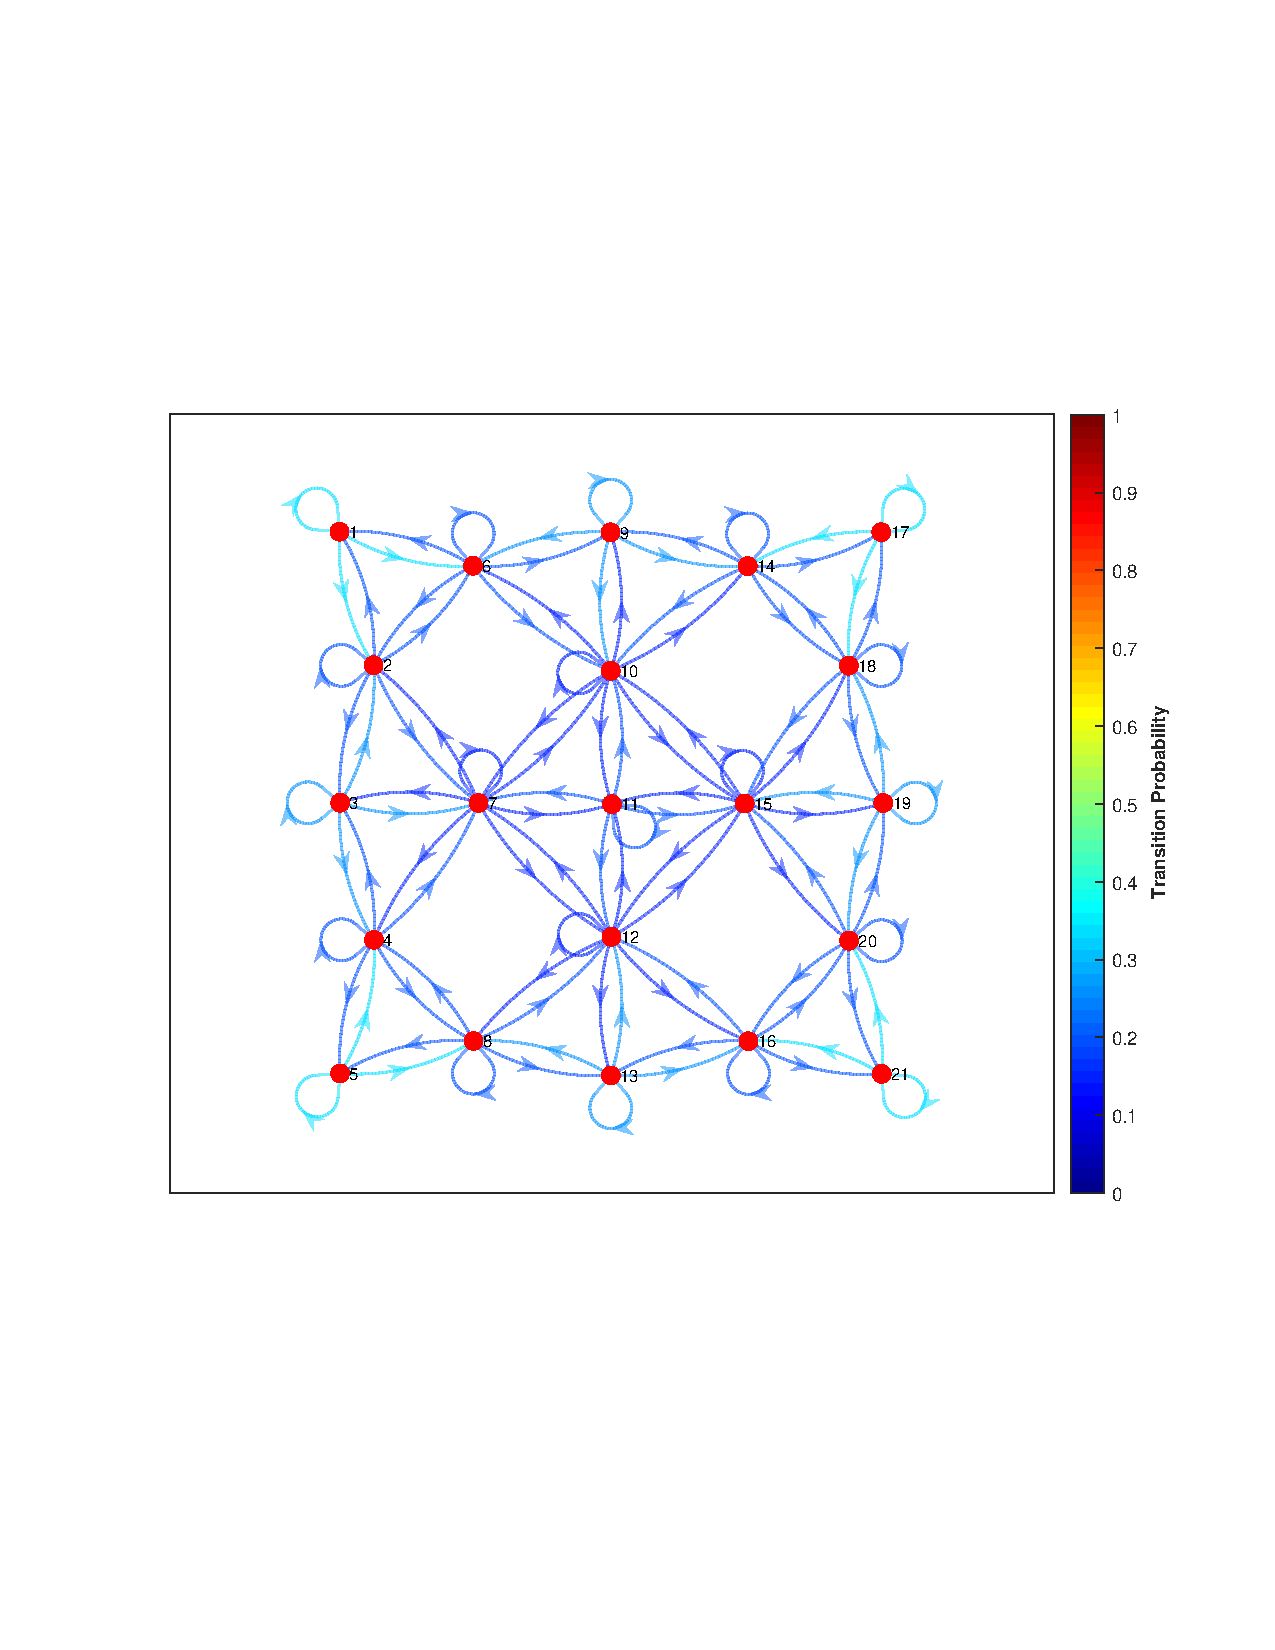
\includegraphics[width=\columnwidth]{./CaseA_MarkovChain_SmallChessboard.pdf}
\caption{A schematic of the model used in case study~\ref{subsec:studyA}.
The Markov Model has 21 states, and is being observed by five agents over an
unreliable network.}
\label{fig:c1a}
\end{figure}

\begin{figure*}
	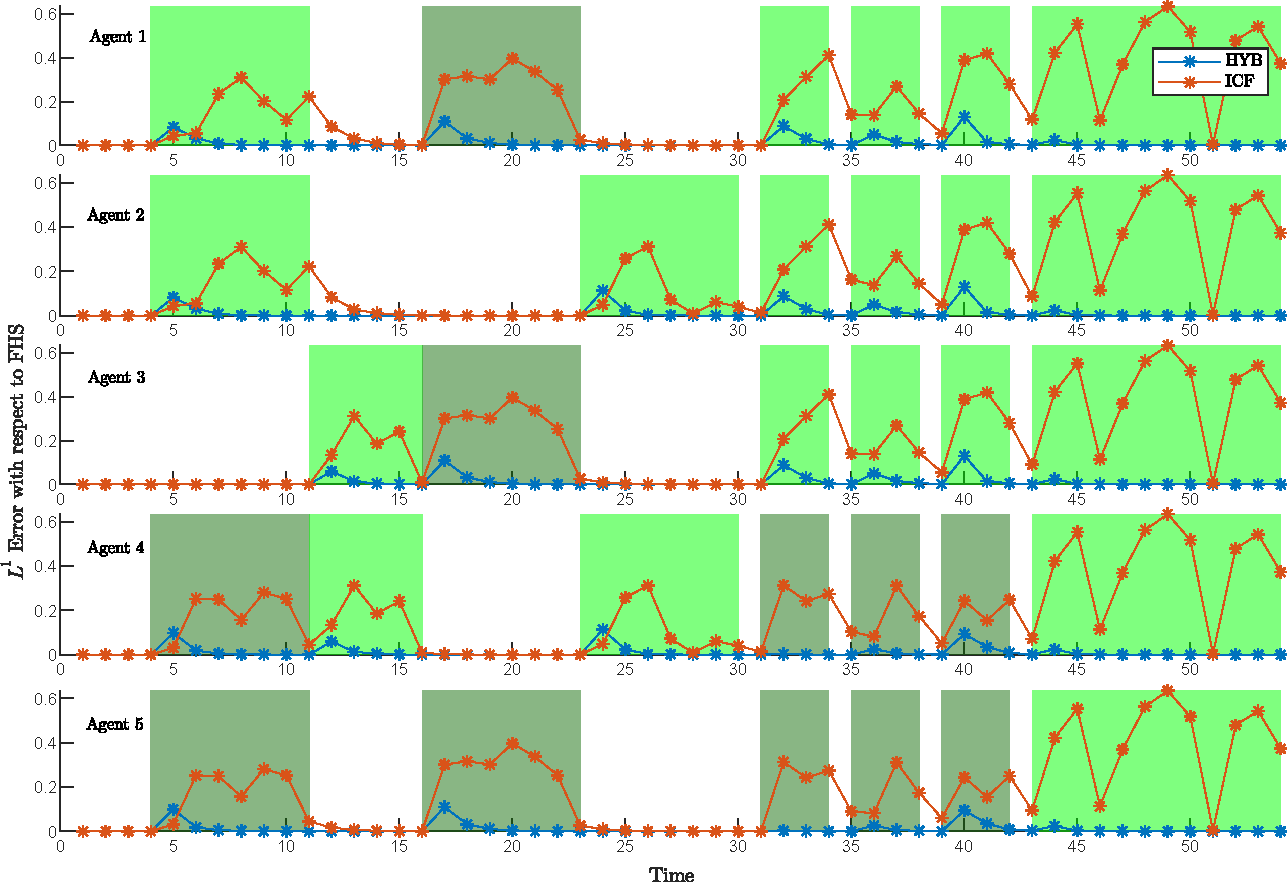
\includegraphics[width=\linewidth]{./CaseA_L1_SmallChessboard.pdf}
\caption{Performance comparison of HYB and ICF on the Markov Model in
Figure~\ref{fig:c1a}.  The shaded areas mark the lifetime of components and
agents with the same shade of color belong to the same component. }
\label{fig:c1b}
\end{figure*}





Then using \eqref{eq:deltaineq} and  \eqref{eq:timeterms},
\begin{align}
\frac{1}{T}\sum_{t=t_0}^{t_0+T}\left\| {}^\suf{FHS}\pi_{t}^{j} - {}^\suf{HYB}\pi_{t}^{j}\right\|_1 &\le
\frac{1}{T}\sum_{k} (2t_{c,k} \delta + t_{c, k} (1-\delta)\epsilon_1) \nonumber \\
& = \frac{1}{T}\sum_{k} t_{c, k} (2\delta + (1-\delta)\epsilon_1) \nonumber \\
& = (2\delta + (1- \delta)\epsilon_1) \frac{1}{T}\sum_{k} t_{c, k} \nonumber \\
& = 2\delta + (1- \delta)\epsilon_1.
\end{align}	
Thus, 
\begin{equation}
\|{}^\suf{FHS}J^{j} - {}^\suf{FHS}J^{j}\|_1 \le L(2\delta + (1-\delta) \epsilon_1).
\end{equation}
Substituting $\delta$ from inequality \eqref{eq:deltaineq} and using \eqref{eq:prop1eq} one can arrive at $N_{\epsilon_2}$ as calculated in  \eqref{eq:neps2}. \end{proof}	



\section{Experiments} \label{sec:experiments}

We conduct an analysis of the comparative performance of our method in two
ways.  First, we examine two case studies (see~\ref{subsec:studyA} and
\ref{subsec:studyB}) which, though abstract, are  representative of
robotic-sensor network applications.  Secondly, we carried out experiments
where we isolated and controlled various parameters, examining the effect they
have on the average performance. 


\subsection{Convergence properties in a generic Markov Chain} \label{subsec:studyA}

In the first case study we consider a system consisting of five agents
connected to each other through a time-varying network. Agents make
observations of the state of a HMM with 21 states.  The transition model of the
HMM is shown in Figure~\ref{fig:c1a}, with transition probabilities represented
by color coded arrows.  The plots in Figure~\ref{fig:c1b} show the performance
of the Hybrid and ICF methods compared to FHS as connected components form and change. The horizontal axis shows the
progression of time;
the vertical axis is the difference between estimated PMF and FHS (measured
with $L^1$ norm). 
The convergence behavior discussed in Remark~\ref{rem:ergodicity} is 
directly visible in the Hybrid method and,
for this system of moderate size, in most cases
convergence takes three steps after the
formation of a component. 
Note also how components with more agents experience faster
convergence.
One particularly salient instance in Figure~\ref{fig:c1b} is the rapid
convergence after step forty-four where the network becomes fully connected.

In contrast, ICF's performance is erratic during connected times possessing
exponential convergence only for agents that are disconnected from the rest of
the network.  This phenomenon can be explained using \eqref{eq:icfprop}, where
we established that, under general conditions, for connected components, $
T^{\suf{FHS}}_{t_{k}:t_{k}+n}\neq T^{\suf{ICF}}_{t_{k}:t_{k}+n}$ except for the
trivial case of a component with single agent. The exponential convergence of
ICF for agent~2 in $t\in[11,24]$ is one such case. The convergence in this
period is due to the forgetting factor of the HMM.


\subsection{A Tracking Example} \label{subsec:studyB}

Our second case study is concerned with a decentralized target pose estimation
problem on a grid using multiple observers connected through a changing
network topology. Figure~\ref{fig:exp1} depicts the 2D grid in which a target
performs a random walk while six observers are trying to estimate its position. 
Each white cell is modeled as a single state of our HMM representing the 
position of the target on the grid. The observers' motion is a deterministic
back-and-forth patrolling route; four of them are rooks moving along the
borders and the other two are bishops moving diagonally on the grid. In order
to detect the target, each observer 
emits a straight beam perpendicular to its direction of motion as shown in the 
figure. The beam either hits the target or an obstacle. In the first case, the 
observer senses the position of the target 
based on a discrete one dimensional Gaussian distribution over the states that 
the beam has traversed; otherwise, under the assumption of no false 
positives, the observer produces a ``no target'' symbol. (The model
has an additional state, which is incorporated into the observation model by
setting zero probabilities in the likelihood matrix for those states that beam
has traveled through to hit a wall.)

\begin{figure}[t]
	\centering
	{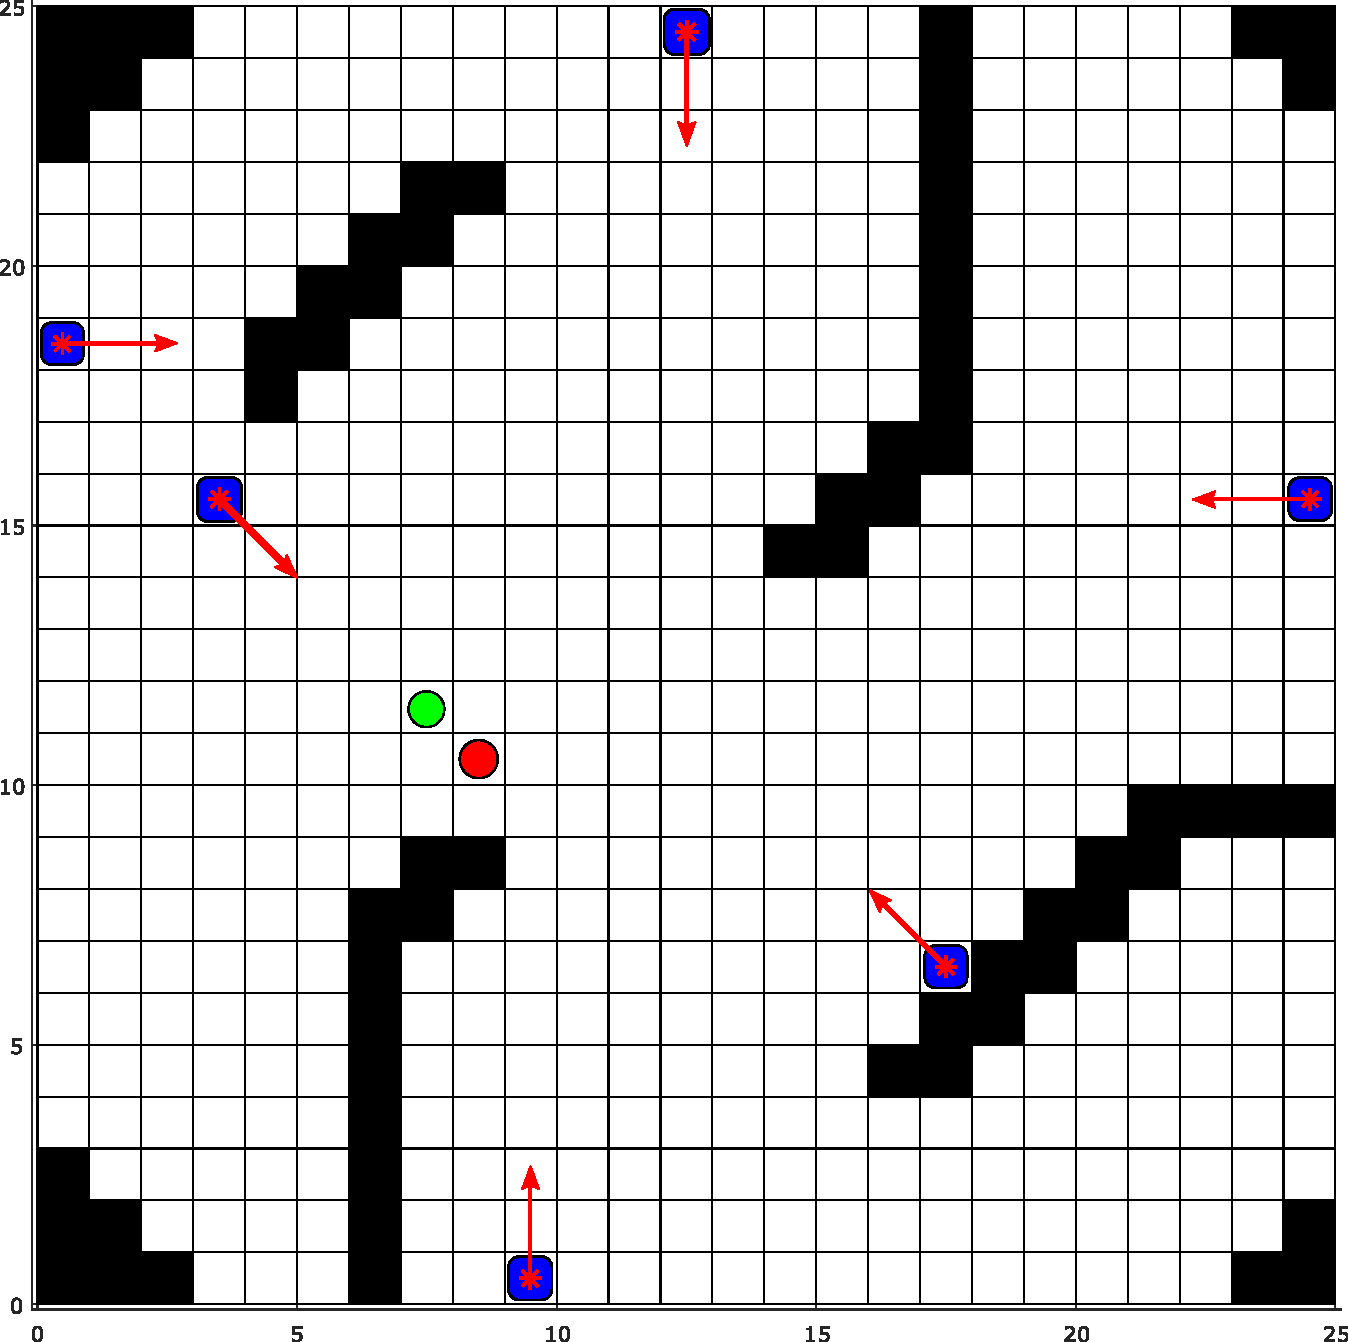
\includegraphics[width=.8\columnwidth]{./exp1_Corrected2.pdf}}
    \caption{The grid-based map of the environment for the tracking
    example~\ref{subsec:studyB}. The dark cells depict obstacles; blue circles
    are trackers and the red circle is the ground truth location of the
    maneuvering target; the green circle depicts an observation made by an
    agent.\label{fig:exp1}}
\end{figure}


For every Markov transition, each observer carries out its decentralized 
estimation step for the position of the target, which is shared with other 
connected observers through a communication network. The network topology
varies randomly resulting in the formation of different connected
components. However, we assume all communications occur at a higher rate than
Markov transition steps, allowing the connected nodes to reach consensus
over the shared information.


\begin{figure*}[t]
\centering
{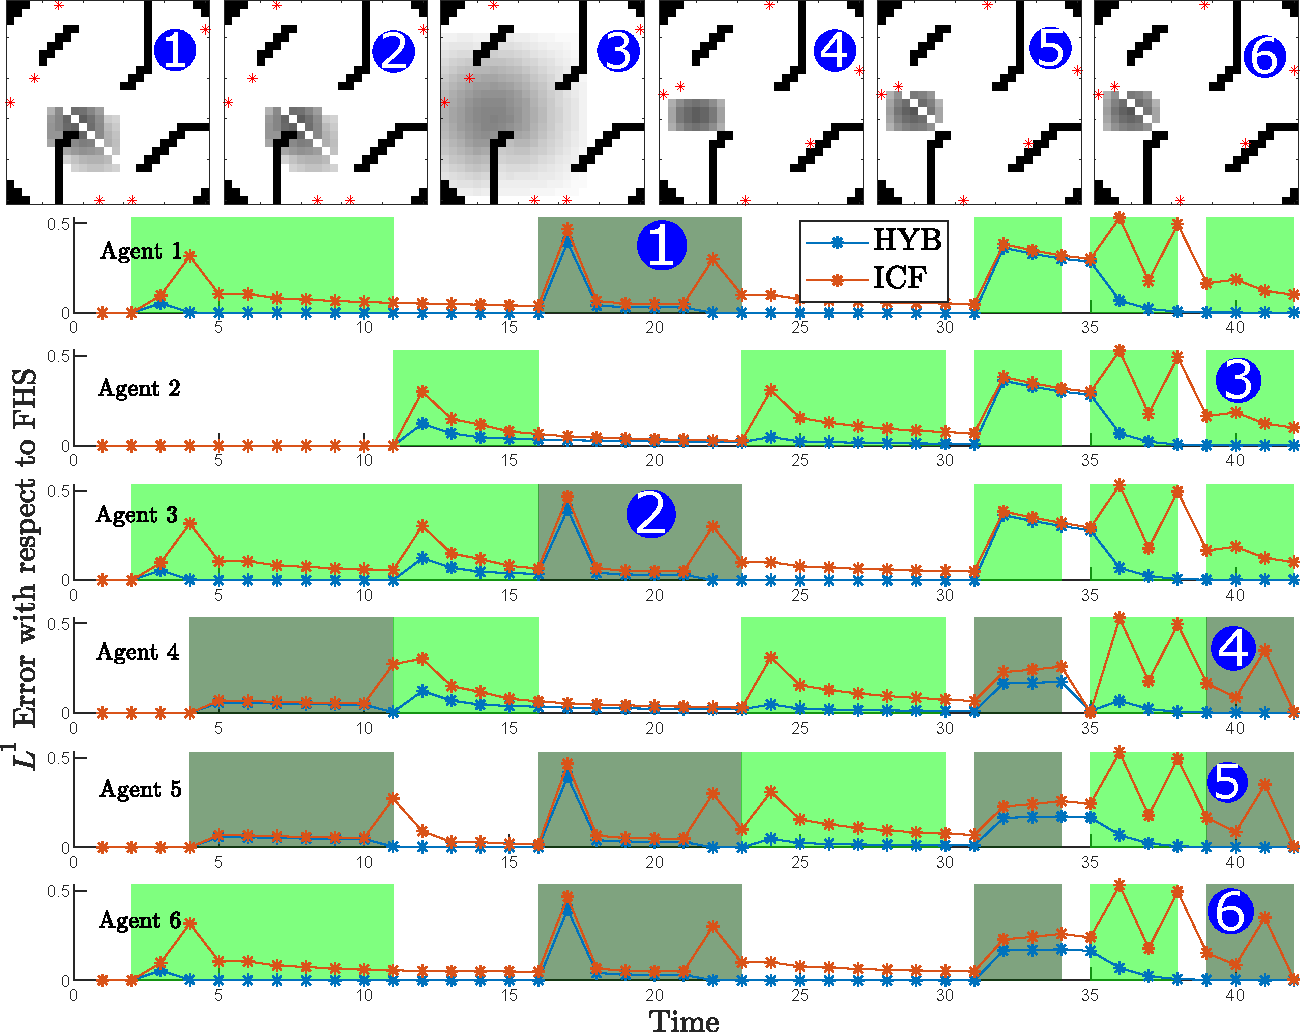
\includegraphics[width=.95\linewidth]{./CaseB_Chessboard_2.pdf}}
\caption{Estimation performance for the tracking case study (see
Figure~\ref{fig:exp1} for the environment and details of the scenario).
For each
agent its distribution at a single step is shown at the top and is indexed
accordingly at its representative time.}
\label{fig:exp2}
\end{figure*} 

We evaluate the performance of the Hybrid method during the phase where the
agents become disconnected from each other, and are then reconnected after some
interval. Similar to the previous case, for purposes of comparison, each agent
performs three estimation processes. In one instance it uses our Hybrid method
to fuse its prior along with the received priors. In the second instance it
uses the ICF method to fuse its posterior along with the received posteriors,
and the third instance is the FHS method, to give a baseline for comparison.
Again, $L^1$ norm difference is used to make the comparison. 

Figure~\ref{fig:exp2} compares the performance of the Hybrid and ICF methods,
showing that the proposed method outperforms ICF and is able to recover
performance very close to FHS solution after reconnection. Using the same
visual presentation as before, the shaded areas mark the lifetime of
components and agents with the same shade color belong to the same component.
Based on the $L^1$ distance, both decentralized estimates converge to FHS
during the interval of network partition. This is expected, since observers do
not have access to each others information and hence, due to the forgetting
property of the system, all three estimators become
indistinguishable---separate agents each performing its own Bayesian update
independently. However, while the Hybrid method is able to start to recover
immediately after reconnection, ICF continues with degraded performance even
after reconnection owing to the fact that it ignores the correlations. 

\begin{figure*}
	\begin{subfigure}{0.50\textwidth}
		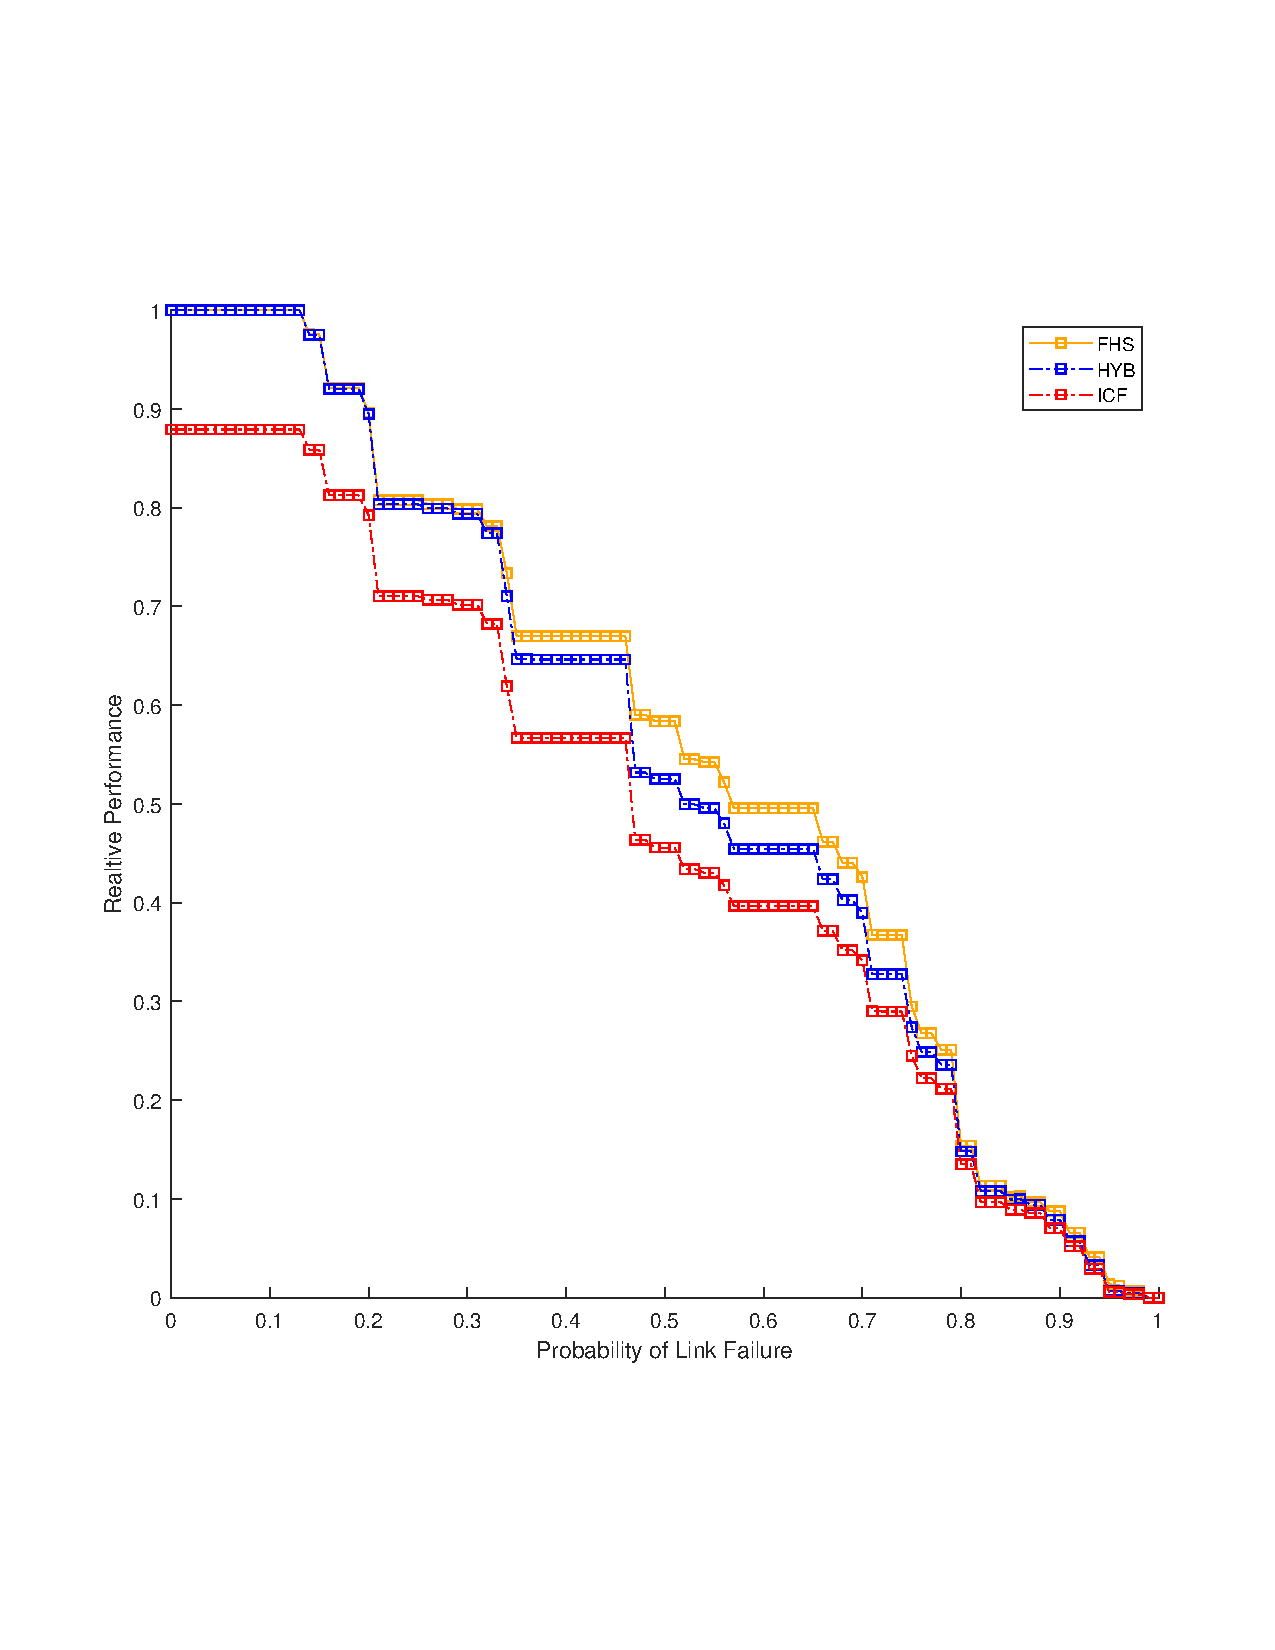
\includegraphics[width=\linewidth]{./CaseC_FigPerf_Chessboard_RndNet.pdf}
		\caption{Average performance for chessboard tracking example} \label{fig:1a}
	\end{subfigure}
	\hspace*{\fill} % separation between the subfigures
	\begin{subfigure}{0.50\textwidth}
		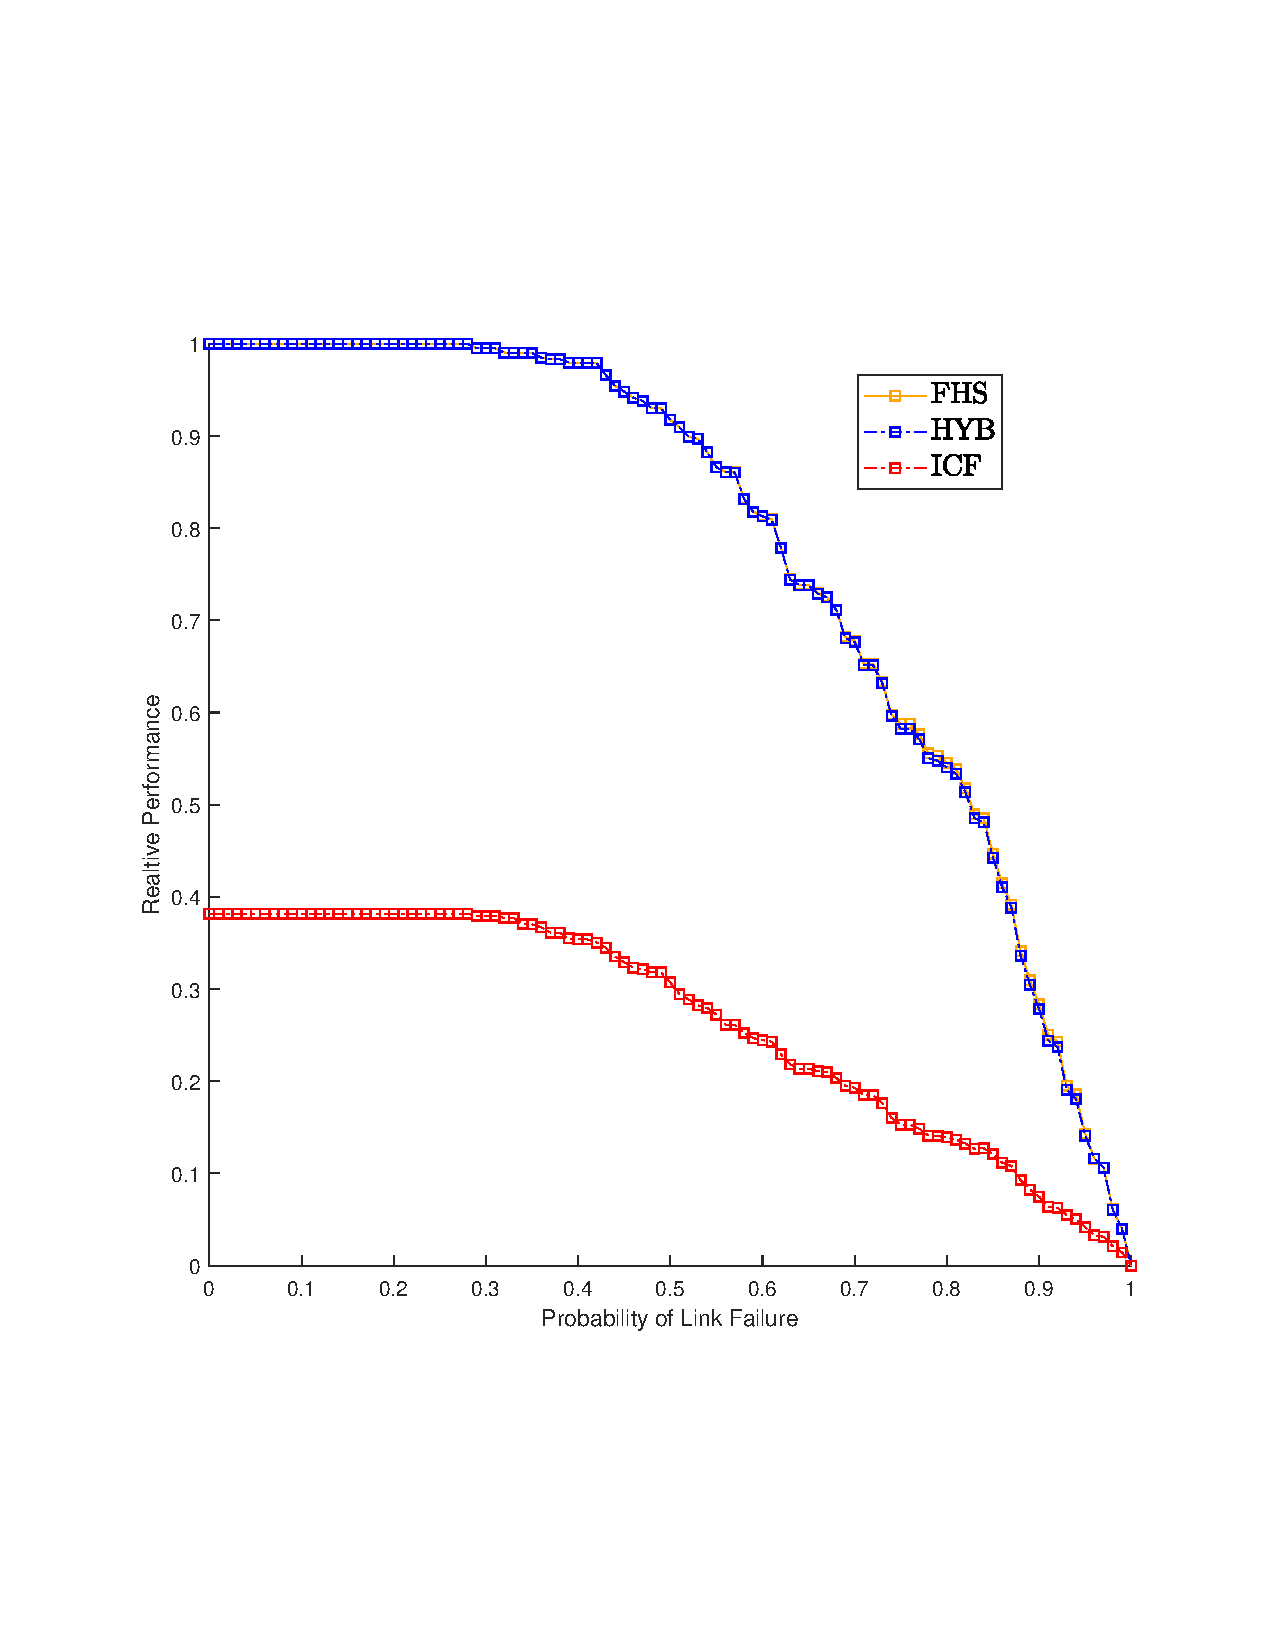
\includegraphics[width=\linewidth]{./CaseC_FigPerf_20N_3S_RndNet.pdf}
		\caption{Average performance for system with three states and twenty observers} \label{fig:1b}
	\end{subfigure}
	\caption{Performance comparison between the Hybrid method and ICF. The horizontal axis   is probability of link failure, moving from left to right represents the network changing 
		from ideal through fragmentation to complete failure. The vertical axis is a metric of estimator performance
		computed as follows: At each time, for every agent, the total variation distance of the estimator's PMF and the output from a hypothetical, omniscient centralized estimator (as if it were operating on a perfect network) is computed. The mean of this is taken over agents and over all times, and then normalized between 0 and 1, where 1 coincides with the fully connected network and 0 the fully disconnected one.
		\label{fig:gcf2}}
\end{figure*}
\balance

\subsection{Controlled Performance Evaluation} \label{subsec:eval}

Next we study the robustness of our method more systematically with respect to
network failure. This permits some reflection on the factors that affect the
gap between the average performance of our method and FHS.  The experiments
reported in this subsection were
performed is as follows.

We take the HMM and construct a fully connected communication network. 
This is the base network topology. We then assign a probability
of link failure  $p$ to all the links in the communication graph and run FHS,
HYB, and ICF methods for 50 steps. At each step we randomly disconnect links
in the base graph with probability $p$  and perform the consensus processes on
the resulting graph. For $\pi^j_k$,  the local estimate of agent $j$ at time
$k$, and $\pi^*_k$, the estimate from the omniscient
estimator,  we compute the instantaneous performance score as 
\begin{equation}
1-\frac{1}{2}\left\| \pi^j_k - \pi^*_k\right\|_1,
\end{equation}
which ensures that scores are within $[0,1]$ interval, where $1$ connotes the
best performance and $0$ the worst. We tally the results for each DSE
variant.
Since even in a fully disconnected network, agents have access to
their own observations, the lowest score is seldom zero. To account
for the specific effects of network degradation (rather than observability of
the HMM itself), we then re-normalize the results to $[0,1]$ interval.  In the
end, we plot the average normalized performance vs. probability of link
failure. The diagram that results gives insight into the robustness of the DSE
method with respect to network failure and gives a clear
visualization of the gap between FHS and other methods. 

Diagrams, as just explained, were constructed for the distributed tracking
example in~\ref{subsec:studyB} and another system consisting of 20
agents observing a HMM with three states.  The results can be seen in
Figures~\ref{fig:1a} and~\ref{fig:1b} respectively.  Some 
observations of interest can be made.

Figure~\ref{fig:1a} shows that the threshold beyond which centralized
estimation is not possible ($p_0= 0.12$) is small for the target tracking
example. Comparing
Figure~\ref{fig:1a} to  Figure~\ref{fig:1b}, the performance gap between ICF
and HYB is smaller, the gap between ICF and FHS is narrower too,
and the decline in performance is sharper. 
This can be explained by the large number of states in the HMM of the
tracking example (559~states) along with the fact that there are only six
observers that track the maneuvering target.  
The result in Figure~\ref{fig:1a} suggests
that the benefit of using Hybrid method over ICF is less pronounced for systems
with less accurate observation models, or on time-varying networks consisting
of many small-sized, short-lived connected components. 

Figure~\ref{fig:1b} illustrates a case where 
there are more observers, $n= 20$, and the
improvement over ICF is drastic
and the gap between HYB and FHS is negligible.  Unlike the tracking problem in
Figure~\ref{fig:1a}, the gap between ICF and HYB is substantial even for values $0 \ll
p$.  That is because for large
connected networks even if some links fail, the size of the connected
components and their lifetime is much longer than those in smaller networks.
This is a property of network reliability and its mathematical foundations
are well-studied but beyond the scope of this paper. For our purposes
it suffices to say that based on the example in  Fig~\ref{fig:1b},  on
reliable networks, the advantage of using Hybrid over ICF is clear.
The results in Figure~\ref{fig:1b} also show that if the ratio of observers to
states is large, Hybrid method performance approaches FHS even
for when the probability of link failure is substantial.

Taking both examples in this subsection together, adopting the Hybrid method
over ICF is always beneficial. Also, the improvement over ICF and the degree to
which the gap with FHS is closed depends on the intrinsic properties of the HMM
and underlying network. 


%%%%%%%%%%%%%%%%%%%%%%%%%%%%%%%%%%%%%%%%%%%%%%%%%%%%%%%%%%%%%%%%%%%
\section{Conclusion} \label{sec:conclusion}

This paper proposes a distributed state estimator for discrete-state dynamic
systems with non-Gaussian noise in networks with changing topology and those
that do not remain connected all the time.  The method is able to achieve
robustness and recover performance after an interval of disconnection.
Separating the process of consensus for the correlated and uncorrelated
information was the key to achieving better performance compared to ICF alone.
Theoretical analysis guarantees that the method proposed in this paper will
show promising convergence properties and outperforms the competitors.  In many
cases, this is by a significant margin.  Evaluating the proposed method in a
series of experiments showed considerable performance improvement compared to
the state of the art in practice.  The experiments also validated the
mathematical analysis, showing exponential convergence under $L_1$ very clearly.

\section*{Acknowledgements}

This work was supported by the National Science Foundation 
in part by IIS-1302393, IIS-1453652, and ECCS-1637889.
%%%%%%%%%%%%%%%%%%%%%%%%%%%%%%%%%%%%%%%%%%%%%%%%%%%%%%%%%%%%%%%%%%%%%%%%%%%%%%%%
\bibliographystyle{IEEEtran} %\bibliographystyle{apalike}
\bibliography{RSS_2017}
%%%%%%%%%%%%%%%%%%%%%%%%%%%%%%%%%%%%%%%%%%%%%%%%%%%%%%%%%%%%%%%%%%%%%%%%%%%%%%%%

\end{document}
